%% To submit your paper:
%DIF LATEXDIFF DIFFERENCE FILE
%DIF DEL manuscripteea6562090c30f4cfa7fca41c1e6bc0675333cbf.tex   Fri Aug 21 15:54:59 2026
%DIF ADD case_for_temperature.tex                                 Fri Aug 21 15:53:44 2026
\documentclass[draft]{agujournal2019}
\usepackage{url} %this package should fix any errors with URLs in refs.
\usepackage{lineno}
\usepackage[inline]{trackchanges} %for better track changes. finalnew option will compile document with changes incorporated.
\usepackage{soul}
\linenumbers
\usepackage{multirow}
\usepackage{amsmath}
\usepackage{amssymb}
\usepackage{siunitx}
\usepackage{booktabs}
\usepackage{xr}
\usepackage{xspace}

\hfuzz=100pt
\hbadness=10000

\externaldocument{supplement}  % no .tex extension

\draftfalse

\journalname{JGR: Atmospheres}

%%%%%%% MAKE SOME COMMANDS %%%%%%%%%%
\newcommand{\eqtn}[1]{Eq.~(\ref{#1})}       % Equation reference
\newcommand{\fig}[2]{\textcolor{red}{(Fig.~\ref{#1}{#2})}}   % Figure reference
\newcommand{\fignop}[2]{\textcolor{red}{Fig.~\ref{#1}{#2}}}  % Figure reference

\newcommand{\todo}[1]{\textcolor{purple}{TODO: #1}}      % Comments
\newcommand{\comment}[1]{\textcolor{cyan}{#1}}     % TODO notes
\newcommand{\mynum}[1]{\textcolor{olive}{#1}}

% meteorological terms go here
\newcommand{\tmin}{\textcolor{black}{$T_{\mathrm{min}}$}\xspace}
\newcommand{\tair}{\textcolor{black}{$T_{\mathrm{air}}$}\xspace}
\newcommand{\tsfc}{\textcolor{black}{$T_{\mathrm{sfc}}$}\xspace}
\newcommand{\qair}{\textcolor{black}{$q_{\mathrm{air}}$}\xspace}
\newcommand{\qsfc}{\textcolor{black}{$q_{\mathrm{sfc}}$}\xspace}
\newcommand{\lwnet}{\textcolor{black}{$LW_{\mathrm{net}}$}\xspace}
\newcommand{\wspd}{\textcolor{black}{$w_{\mathrm{spd}}$}\xspace}
\newcommand{\wdir}{\textcolor{black}{$w_{\mathrm{dir}}$}\xspace}
\newcommand{\cloudfrac}{\textcolor{black}{$C_{\mathrm{frac}}$}\xspace}
\newcommand{\dq}{\textcolor{black}{$\Delta q$}\xspace}
\newcommand{\dT}{\textcolor{black}{$\Delta T$}\xspace}
\newcommand{\fq}{\textcolor{black}{$F\mathrm{_q}$}\xspace}
\newcommand{\ustar}{\textcolor{black}{$u_{\star}$}\xspace}
\newcommand{\lwup}{\textcolor{black}{$LW\uparrow$}\xspace}
\newcommand{\lwdn}{\textcolor{black}{$LW\downarrow$}\xspace}
\newcommand{\tsnow}{\textcolor{black}{$T_{\mathrm{snow}}$}\xspace}
\newcommand{\qsnow}{\textcolor{black}{$q_{\mathrm{snow}}$}\xspace}
\newcommand{\pbaro}{\textcolor{black}{$P_{\mathrm{baro}}$}\xspace}
\newcommand{\rnet}{\textcolor{black}{$R_{\mathrm{net}}$}\xspace}
\newcommand{\hs}{\textcolor{black}{H$_s$}\xspace}
\newcommand{\hlat}{\textcolor{black}{H$_l$}\xspace}
\newcommand{\swnet}{\textcolor{black}{$SW_{\mathrm{net}}$}\xspace}
\newcommand{\swdn}{\textcolor{black}{$SW\downarrow$}\xspace}
\newcommand{\swup}{\textcolor{black}{$SW\uparrow$}\xspace}
\newcommand{\dcc}{\textcolor{black}{$\Delta$CC}\xspace}
\newcommand{\albedo}{\textcolor{black}{$\alpha$}\xspace}
\newcommand{\rfalb}{\textcolor{black}{RF$_{albedo}$}\xspace}
\newcommand{\rfcirrus}{\textcolor{black}{RE$_{cloud}$}\xspace}
\newcommand{\rfcanopy}{\textcolor{black}{RF$_{canopy}$}\xspace}


% units
\newcommand{\um}{\textcolor{olive}{$\mu$m}\xspace}
\newcommand{\ms}{\textcolor{olive}{m$\cdot$s$^{-1}$}\xspace}
\newcommand{\gkg}{\textcolor{olive}{g$\cdot$kg$^{-1}$}\xspace}
\newcommand{\kmsq}{\textcolor{olive}{km$^2$}\xspace}  % kilometers
\newcommand{\wmsq}{\textcolor{olive}{W$\cdot$m$^{-2}$}\xspace}
\newcommand{\degr}{\textcolor{olive}{$^\circ$}\xspace}
\newcommand{\degrc}{\textcolor{olive}{$^\circ$C}\xspace}
\newcommand{\gmtwo}{\textcolor{olive}{gm$^{-2}$}\xspace}
\newcommand{\kgmtwo}{\textcolor{olive}{kg$\cdot$m$^{-2}$}\xspace}
\newcommand{\mjmtwo}{\textcolor{olive}{MJ$\cdot$m$^{-2}$}\xspace}
%DIF PREAMBLE EXTENSION ADDED BY LATEXDIFF
%DIF UNDERLINE PREAMBLE %DIF PREAMBLE
\RequirePackage[normalem]{ulem} %DIF PREAMBLE
\RequirePackage{color}\definecolor{RED}{rgb}{1,0,0}\definecolor{BLUE}{rgb}{0,0,1} %DIF PREAMBLE
\providecommand{\DIFadd}[1]{{\protect\color{blue}\uwave{#1}}} %DIF PREAMBLE
\providecommand{\DIFdel}[1]{{\protect\color{red}\sout{#1}}}                      %DIF PREAMBLE
%DIF SAFE PREAMBLE %DIF PREAMBLE
\providecommand{\DIFaddbegin}{} %DIF PREAMBLE
\providecommand{\DIFaddend}{} %DIF PREAMBLE
\providecommand{\DIFdelbegin}{} %DIF PREAMBLE
\providecommand{\DIFdelend}{} %DIF PREAMBLE
\providecommand{\DIFmodbegin}{} %DIF PREAMBLE
\providecommand{\DIFmodend}{} %DIF PREAMBLE
%DIF FLOATSAFE PREAMBLE %DIF PREAMBLE
\providecommand{\DIFaddFL}[1]{\DIFadd{#1}} %DIF PREAMBLE
\providecommand{\DIFdelFL}[1]{\DIFdel{#1}} %DIF PREAMBLE
\providecommand{\DIFaddbeginFL}{} %DIF PREAMBLE
\providecommand{\DIFaddendFL}{} %DIF PREAMBLE
\providecommand{\DIFdelbeginFL}{} %DIF PREAMBLE
\providecommand{\DIFdelendFL}{} %DIF PREAMBLE
%DIF COLORLISTINGS PREAMBLE %DIF PREAMBLE
\RequirePackage{listings} %DIF PREAMBLE
\RequirePackage{color} %DIF PREAMBLE
\lstdefinelanguage{DIFcode}{ %DIF PREAMBLE
%DIF DIFCODE_UNDERLINE %DIF PREAMBLE
  moredelim=[il][\color{red}\sout]{\%DIF\ <\ }, %DIF PREAMBLE
  moredelim=[il][\color{blue}\uwave]{\%DIF\ >\ } %DIF PREAMBLE
} %DIF PREAMBLE
\lstdefinestyle{DIFverbatimstyle}{ %DIF PREAMBLE
	language=DIFcode, %DIF PREAMBLE
	basicstyle=\ttfamily, %DIF PREAMBLE
	columns=fullflexible, %DIF PREAMBLE
	keepspaces=true %DIF PREAMBLE
} %DIF PREAMBLE
\lstnewenvironment{DIFverbatim}{\lstset{style=DIFverbatimstyle}}{} %DIF PREAMBLE
\lstnewenvironment{DIFverbatim*}{\lstset{style=DIFverbatimstyle,showspaces=true}}{} %DIF PREAMBLE
%DIF END PREAMBLE EXTENSION ADDED BY LATEXDIFF

\begin{document}

\title{The Snow Energy Balance During Extreme Ablation: A Case Study of the March 2026 Heatwave in the Sierra Nevada}

\authors{William Rudisill\affil{1}, Alan Rhoades\affil{1}, Megan Mason\affil{2}, Gabriel Lewis\affil{2}, Andrew Schwartz\affil{2}, Marianne Cowherd\affil{4}, Benjamin Hatchett\affil{3}, Erica Siriila-Woodburn\affil{1}, Dan Feldman\affil{1}}

\affiliation{1}{Lawrence Berkeley National Laboratory, Earth and Environmental Sciences Area}
\affiliation{2}{UC Berkeley Central Sierra Snow Laboratory}
\affiliation{3}{Colorado State University}
\affiliation{4}{Montana State University}
%(repeat as many times as is necessary)

\correspondingauthor{William Rudisill}{williamrudisill@lbl.gov}

\begin{keypoints}
\item Record heat coincided with record \DIFaddbegin \DIFadd{snow drought and }\DIFaddend rates of snow ablation during March of \DIFdelbegin \DIFdel{2026, leading to record low-to-no-snowpack conditions.
}\DIFdelend \DIFaddbegin \DIFadd{2026.
}\DIFaddend \item Net-shortwave was the dominant ablation driver despite the anomalously warm air temperatures. 
\item Low snow-albedo and higher than average downwelling shortwave\DIFdelbegin \DIFdel{due to a lack of mid level clouds}\DIFdelend \DIFaddbegin \DIFadd{, caused by an anomalous lack of mid-level clouds, }\DIFaddend contributed to record rates of net-shortwave of the snowpack.
\item Snow ablated more slowly under vegetation canopy due to enhanced solar shading. 
\item Less than \DIFdelbegin \DIFdel{\todo{x} }\DIFdelend \DIFaddbegin \DIFadd{1\% }\DIFaddend of total snow ablation was due to sublimation\DIFaddbegin \DIFadd{, lower than the climatological average}\DIFaddend .
\item Boundary layer decoupling and vapor pressure arguments explain the small contribution of sensible heating and sublimation to the snow energy and mass balance during the \DIFdelbegin \DIFdel{heatwaves}\DIFdelend \DIFaddbegin \DIFadd{heatwave}\DIFaddend .

\end{keypoints}

\begin{abstract}
Test
\end{abstract}

\section*{Plain Language Summary}
Enter your Plain Language Summary here or delete this section.


\section{Introduction}
While meltwater from seasonal snowpacks has historically provided $\sim$70\% of runoff in the western USA \cite{Li2017-dj}, these natural reservoirs and our ability to measure, monitor, and predict them are in decline \cite{Hale2023-kx, Cowherd2024-zm}.
From a practical perspective, many operational snowmelt runoff models use a temperature index approach, whereby air temperature (\tair) is the primary predictor of melt \cite{Anderson1973-jx}.
While these models have proven effective, the physical justification for such models is not clear.
Since at least the 1980s\DIFaddbegin \DIFadd{, }\DIFaddend the field of snow hydrology appreciates that understanding the climatic behavior of snow necessitates considering the entire energy budget of the snowpack.
In particular, it is well accepted that the net shortwave radiation absorbed by the snowpack (\swnet) is a first-order predictor of rates of melt \cite{Marks1992-qo, Cline1997-de}.
Both small impurities \cite{Deems2013-vv} and wet and dry grain-growth mechanisms \cite{Colbeck1982-gv} tend to decrease the amount of reflected sunlight (the snow albedo, \albedo) and are responsible, in conjunction with rising sun-angles, for the large increases in \swnet in the spring.
Unlike downwelling longwave (\lwdn; 4--100\um), the downwelling component of shortwave (\swdn; 0.3--3\um) is mainly insensitive to variations in \tair itself.
Variations in \swdn in time (and across elevation) are driven primarily by Rayleigh scattering by O$_2$ and N$_2$, Mie scattering by natural occurring and human-made aerosols, dust, and cloud droplets, as well as absorption primarily by water vapor, CO$_2$, and O$_3$.

% recent heatwave work
At the same time, recent work has highlighted the strong correlation between extreme snow ablation (the loss of snow to either sublimation or melt) events and so-called ``snow-eater heatwaves'' --- prolonged periods of sustained (day and night), anomalous, and above freezing \tair during the snow season \cite{Rhoades2026-jm}.
The characteristics of snow-eater heatwaves have already appreciably changed since the 1850s.
These events are occurring more frequently, at a higher intensity, over a larger portion of the western US (WUS), and earlier in the water year.

%These with warming in addition to the mean-annual air temperature.
An example of such an early-season, high-intensity, snow-eater heatwave (SEHW) occurred in March of 2026, when the monthly March \tair across the WUS \DIFdelbegin \DIFdel{were }\DIFdelend \DIFaddbegin \DIFadd{was }\DIFaddend 3 standard deviations above long-term averages observed at many stations.
Recent rapid-attribution studies have shown the snow loss associated with this event is \todo{X to Y} \% more likely due to anthropogenic climate change.
This event (which started earlier than the window of occurrence studied in \citeA{Rhoades2026-jm}) resulted in widespread and rapid ablation at many snow-observing sites\DIFdelbegin \DIFdel{and }\DIFdelend \DIFaddbegin \DIFadd{, and streamflow that was }\DIFaddend one-to-two \DIFdelbegin \DIFdel{month }\DIFdelend \DIFaddbegin \DIFadd{months }\DIFaddend earlier than average \DIFdelbegin \DIFdel{streamflow }\DIFdelend in many watersheds.
This raises an apparent paradox: if \swdn provides most of the energy for snowmelt, and yet it is largely insensitive to \tair, then why are heatwaves so efficient at ablating snow?

% It has been argued that their efficacy arises not from the relationship between \tair and turbulent fluxes of sensible heat into the snowpack, but rather the relationship between longwave radiation (\lwdn) emitted by the atmosphere \citep{Pluss1997-wx, Ohmura2001-ll}.
% % \cite{Brutsaert1975-jl} showed that \todo{the radiative transfer equations reduce to .... }.

% what are we going to do
Using the March 2026 event as a case study, we ask the following questions:
\begin{itemize}
  \item What are the dominant snowmelt energy forcings during early-season heatwaves, and how do they scale with increasing \tair?
  \item How do vegetation canopies and atmospheric conditions --- including clouds or lack thereof --- shape such energetic forcings during heatwave events?
  \item What are the relative contributions of sublimation and melt to extreme snow ablation during such events?
\end{itemize}

% why we should care about veg
For some perspective, approximately half of North America's snow water volume resides under tree canopy \cite{Kim2021-eu}.
Canopies absorb/scatter SW radiation, increase LW radiation, and reduce winds relative to open or non-vegetated snow surfaces; however, the magnitudes of these changes can vary widely across space and time.
A number of studies have considered the effects of vegetation and forest treatments on the mean-state of the snow climate of this region, and it is well observed that snow tends to accumulate more and ablate later in the year in open regions relative to forested regions \cite{Harpold2020-rc, Krogh2020-dh}.
Synthesis work has shown that open versus subcanopy snow dynamics are dependent on latitude and mean winter \tair \cite{Lundquist2013-uc}.
However, the interactions between vegetation and discrete extreme heatwave events \DIFdelbegin \DIFdel{has }\DIFdelend \DIFaddbegin \DIFadd{have }\DIFaddend not previously been considered.

% clouds
Despite otherwise drier-than-normal conditions, high-altitude cirrus clouds can occur during high-pressure ridging events commonly associated with cool-season heatwaves (\citeA{Rhoades2026-jm} Figure 1 and Supplemental Figure S5)\DIFdelbegin \DIFdel{, however}\DIFdelend \DIFaddbegin \DIFadd{; however, }\DIFaddend such events may preclude the formation of low or \DIFdelbegin \DIFdel{midlevel }\DIFdelend \DIFaddbegin \DIFadd{mid-level }\DIFaddend clouds, which have the largest impact on the snow energy balance \cite{Rudisill2025-cx} and are generally \DIFdelbegin \DIFdel{assosciated }\DIFdelend \DIFaddbegin \DIFadd{associated }\DIFaddend with reducing rates of snow ablation\DIFaddbegin \DIFadd{.
}\DIFaddend Frameworks for investigating interactions between clouds and surface radiation are well explored in the literature, using satellite retrievals and surface radiation data \cite{Ramanathan1989-pa, Shupe2004-kl, L-Ecuyer2019-my}, but little work has investigated the extent to which clouds or the lack-thereof contribute to anomalous snow ablation in mid-latitude regions.

% outcomes
The outcomes from this study answer basic science questions about energy available for snowmelt or sublimation in water-resource critical basins in the Sierra Nevada, with implications for other regions.
The findings can directly inform efforts towards management and resilience against extreme events by providing actionable steps towards improving the monitoring and prediction of snowmelt.
Last, improved understanding of vegetation and snow interactions during heatwaves can inform headwater management practices through improved decision support tools (e.g., \citeA{Heggli2026}).


\section{Background and Methods}
% justify using one site
This work is based around in-situ observations collected at the Central Sierra Snow Laboratory (CSSL; \citeA{Schwartz_Cowherd_McGurk_Mason_Riker-Coleman_Zutter_Lewis_2026}), described in the Sec. \ref{sec:study_area}.
Geographic controls on snow processes undoubtedly shape heatwave responses --- but modeling these effects adds inherent uncertainties given the difficulty of distributing forcings across complex terrain \todo{CITE}, which is why we choose to focus on one intensively monitored site.

% what we do
First, we place the record March 2026 heat and associated snow ablation in a climatic and synoptic context, using reanalysis data, remote sensing, and station observations (described in Sec. \ref{sec:observational_data} and \ref{sec:reanalysis_data}).
To explain energy balance anomalies leading to the March ablation, we run single-point configurations of the Structure for Unifying Multiple Modeling Alternatives \cite{Clark2015-ni} from 2000-2026 (described in Sec. \ref{sec:models:summa}) for a forested and open site.
Snow energy balance anomalies are interpreted in reference to historical March conditions for each site.
Sec. \ref{sec:snow_seb}\DIFdelbegin \DIFdel{—}\DIFdelend --\ref{sec:canopy_influence} reviews the snow energy balance and effects of canopy, and Sec. \ref{sec:methods:radforce} details the methods to quantify the contribution to ablation by radiative processes.



\subsection{Study area}\label{sec:study_area}
We focus our analysis on three basins in the immediate vicinity of the Central Sierra Snow Laboratory (CSSL; 39.32 $^\circ$N, 120.37 $^\circ$W, 2100 m.a.s.l) located in Soda Springs, CA  \cite{Schwartz_Cowherd_McGurk_Mason_Riker-Coleman_Zutter_Lewis_2026}.
These include the Yuba, North Fork American, and Truckee River Watersheds (the greater Truckee River Watershed is composed of the Lake Tahoe basin and Truckee River basin at the eight-digit hydrologic unit code (HUC8) scale) \fig{fig:region_map}{a--d}.
The Yuba and North Fork American rivers support the New Bullards Bar and Folsom reservoirs, respectively.
These reservoirs have combined storage capacities approaching 2 million acre feet and hydropower generation potential of 559 megawatts \todo{citation}.
All three rivers support varied downstream consumptive uses (i.e., urban, industrial and agricultural) and provide critical aquatic and riparian habitats.


\subsection{Observational data}\label{sec:observational_data}
% snotel and USHCRN
We use data from twelve Natural Resources Conservation Service (NRCS) SNOwpack TELemetry (SNOTEL) Network stations located throughout the study region spanning \todo{X} to \todo{Y} m.a.s.l.
SNOTEL is the primary snow observing program in the WUS \cite{Serreze1999-as} and routinely measures snow water equivalent (SWE), precipitation, and \tair, though the homogeneity of \tair measurements remains a challenge for the SNOTEL network \cite{Oyler2015-by, McAfee2019-mt}.
To supplement SNOTEL temperature records, we use data from four US Historical Climate Reference Network (USHCRN) stations and the gridded nClimGrid product throughout the study region.
USHCRN stations are high-quality stations subset from the larger GHCN-D dataset \citeA{Menne2012-uu}.
The HCNv2 dataset provides homogenized and quality-assured monthly \tair based on USHCRN data that dates as far back as the  late 1800s \cite{Menne2009-ushcn}.
While \DIFdelbegin \DIFdel{this data does }\DIFdelend \DIFaddbegin \DIFadd{these data do }\DIFaddend not have the same spatial density and elevation range as SNOTEL, the longer temporal record and high quality control mean that these observations can more confidently be used for evaluation of climate extremes, such as heatwave events \cite{BercosHickey2022}.

% csssl
In addition to hosting an NRCS SNOTEL site, CSSL provides long-term meteorological and snowpack records in addition to surface energy balance measurements.
Campbell Scientific CNR4 four-component radiometers measure incoming ($\downarrow$) and outgoing ($\uparrow$) SW and LW radiation from the atmosphere and snowpack.
A Campbell Scientific IRGASON eddy covariance system measures sensible (H$_s$) and latent (H$_l$) heat fluxes above the snowpack.
The CSSL forest study site hosts an additional meteorological station approximately 150 m north of the main CSSL site.
This tower hosts an additional Kipp and Zonen SP Lite2 radiometer that measures below-canopy SW radiation.
SWE measurements were obtained using a federal sampler \cite{Osterhuber2014-ic} at nine discrete sampling intervals during the March heatwave in the forest location.
To maintain temporally and serially complete records and to compare against \DIFdelbegin \DIFdel{climatalogical }\DIFdelend \DIFaddbegin \DIFadd{climatological }\DIFaddend March conditions at this site, this work relies primarily on energy balance model estimates from SUMMA, which we validate in detail against all-available CSSL energy balance fluxes when available (Sec. \ref{supp:sec:validation}).

% Both the IRGASON and CNR4 are hosted on a movable arm \fig{fig:region_map}{c} that automatically adjusts to maintain a constant distance of approximately one meter above the snow surface as snow accumulates or ablates throughout the season.



\subsection{Atmospheric structure and radiation data}\label{sec:reanalysis_data}
% era5 and other data
To investigate the synoptic patterns associated with the March heatwave, we use 500 hPa geopotential height and atmospheric column information from the fifth-generation ECMWF Reanalysis (ERA5) \cite{Hersbach2020-era5}.
Daily geopotential height anomalies during the event are computed using data provided by \citeA{Lee2023-cc}, which has been de-trended and covers the period from 1979 to 2022.

% radiation
We use the Clouds and the Earth's Radiant Energy System (CERES) EBAF, hereafter CERES-EBAF \cite{Kato2018-pi} to investigate the effects of clouds or lack-thereof on the snow energy balance.
CERES-EBAF provides gold-standard measurements of surface and top-of-atmosphere (TOA) irradiances at a 1x1 degree resolution at a monthly cadence.
This product is suitable for trend analysis.
\citeA{Rudisill2025-cx} compared cloud radiative effects from CERES products against in-situ radiometers collected by the SAIL field campaign in the Colorado Rockies \cite{Feldman2023-gp}  and found good agreement, despite grid-resolution mismatches and confounding effects of terrain.
\citeA{Hinkelman2015-ri} likewise found the lower level, hourly CERES-SYN1Deg \cite{Rutan2015-ar} product proved efficacious when used as forcings for snow simulations. 
The 2000--present period-of-record of CERES-EBAF is used to examine the March anomaly in \swdn and \lwdn and the contribution of clouds to the anomalies therein.

%  and CERES-SYN1Deg \cite{Rutan2015-ar},
% CERES-SYN1Deg is a lower-level product that provides hourly estimates of the same quantities but is not configured to examine long-term temporal trends.
% Thus, we use CERES-SYN1Deg all-sky and clear-sky \swdn and \lwdn (e.g., hypothetical irradiance in the absence of clouds) to compute cloud-radiative effects following \citeA{Ramanathan1989-pa} and subsequent studies.

\subsection{SUMMA model configuration}\label{sec:models:summa}
% summa
To investigate the snow energy balance, we use the SUMMA model \cite{Clark2015-ni}.
SUMMA is well-vetted for a range of snow climate applications and provides several options for flux stability corrections, canopy radiation interactions, snow-layering schemes, and other model structural options \cite{Cristea2022-ys}.
We use the Jordan snow layering option, which allows for up to 100 snow layers, the UEB-2 stream approximation for canopy radiation interactions, the ``Louisinv'' option for stability correction of turbulent fluxes, and the ``stickySnow'' canopy snow interception scheme.
SUMMA solves for a vegetation energy balance and canopy air-space temperature which is used to produce \lwdn incident onto the sub-canopy snowpack.
Additional specific modeling parameterizations with relevance to this study are described in Sec. \ref{sec:snow_seb} and the Supplemental Material.
We assign a measurement height of 12m for the model forcings into SUMMA in order to intercompare the effects of 10m tall needleleaf vegetation characteristic of the forest site at CSSL using the same forcing variables.

% more data
We use hourly ERA5 data \cite{Hersbach2020-era5} as SUMMA model forcings after adjusting to the CSSL site.
Daily precipitation from the NRCS SNOTEL site is used directly as forcing when available.
Hourly ERA5 two-meter \tair are bias corrected to match the monthly average \tair observed at the CSSL from the NRCS records by removing a constant linear bias term.
Comparing ERA5 \swdn data to observations from the CNR4 shows good agreement except for morning and evening when the surrounding vegetation  blocks direct beam solar radiation.
To account for this effect, we compute and apply a \swdn correction coefficient as a function of the solar zenith and azimuth angles to adjust the ERA5 data to account for shadows (see Figure \ref{fig:supp_fig_SWd_adjust_sza_azm}).
To ensure that the ERA5 data matches the best available estimates of variability and trends in radiation at this site, we use a multiplicative scale that forces the ERA5 \swdn and \lwdn monthly anomalies to match monthly anomalies in the CERES-EBAF data.
Other forcing variables compared favorably against the available observations and were not adjusted.
Additional information about SUMMA validation is provided in the Supplemental Material (Sec. \ref{supp:sec:validation}).




% RRTMG
% High-level cirrus clouds were observed by the Moderate Resolution Imaging Spectroradiometer (MODIS) satellite imagery at various times during the March 2026 heatwave.
% To model the effects of cirrus clouds on the surface radiation balance, we use the RRTMG radiative transfer model \citep{Iacono2008-ax}, building off work from a previous study \citep{Rudisill2025-cx}.
% We configure RRTMG with one hundred equally spaced pressure levels from the surface (~800hPa at CSSL) to 1 hPa.
% Ozone, water vapor, and thermodynamic profiles for the March 2026 heatwave are acquired from ERA5 for the grid cell encompassing CSSL.

% We define a cirrus cloud radiative effect (cCRF) as the difference between \rnet at the land surface from a cloudy atmosphere against an equivalent, hypothetical clear sky atmosphere following \cite{Ramanathan1989-pa} and subsequent studies.
% To compute cCRF (Table \ref{tab:radiative_effects}), we run RRTMG twice (Sec. \ref{sec:models:rrtmg}).
% First, we run the model with ERA5 thermodynamic profiles and no clouds for the month of March 2026.
% The cirrus cloud properties are described in the supplemental material.
% The purpose of this experiment it to provide a theoretical bound on potential cirrus radiative forcing during the heatwave, rather than a quantitative estimate of the integrated cCRE during the event, which would require estimating/retrieving cirrus properties and frequency throughout the duration of the event.


\subsection{The snow energy balance}\label{sec:snow_seb}
Using meteorological sign conventions for turbulent fluxes, the energy budget of a snowpack is given by:
\begin{align}\label{eq:energy_budget}
\mathrm{Melt}/ \mathrm{Refreeze}  - \Delta\mathrm{CC}
&=
\underbrace{
    H_\mathrm{s} + H_\mathrm{l}
}_{\text{turbulent fluxes}}
+
\underbrace{
LW\downarrow- \sigma\epsilon T_{snow}^4
}_{\text{net longwave}}
+
\underbrace{
   SW\downarrow(1-\alpha)
}_{\text{net shortwave}}
+
G
\end{align},

where Melt/Refreeze is the rate of melt or liquid water refreezing in mass per second multiplied by the latent heat of fusion, $\Delta$CC is the time rate-of-change in the snowpack cold-content \cite{Jennings2018-wz}, $H_s$ and $H_l$ are the turbulent fluxes of sensible and latent heat respectively at the snow/atmosphere interface, $T_{air}$ is the temperature of the air, $T_{snow}$ is the temperature of the snow surface, $\epsilon$ is the emissivity of the snow (0.98), \swdn is the downwelling shortwave radiation, and $\alpha$ is the albedo of the snow surface defined as the ratio of upwelling shortwave radiation (\swup) to \swdn.

% how SWE is related to melt
The mass-balance of the snowpack is related to the energy balance (Eq. \ref{eq:energy_budget}) in the following ways.
The daily or monthly change in SWE (referred to as $\Delta$SWE) is related to both Melt and to a lesser extent $H_l$, though the latter may remove 10\% to upwards of 28\% of the seasonal snow mass depending on a variety of factors \cite{Sexstone2018-rc, Schwat2025-ur}.
Melt may be either positive (melt) or negative (refreezing) using the sign convention in Eq. \ref{eq:energy_budget}.
Melt integrated throughout an entire day is not synonymous with a loss in SWE, since meltwater may be retained in the snowpack and may refreeze or remain in place by tension. 
For flow through the bottom boundary of the snowpack, the dry pore space of the snow must be filled with liquid water to residual saturation \cite{Colbeck1976-xk, Seligman2014-kc}. Snowpacks may retain between 2--8\% liquid water by volume.
In the SUMMA model, meltwater flow throughout the snowpack layers is modeled as a gravity-driven power law; preferential flow is not considered.




\subsubsection{The influence of canopy}\label{sec:canopy_influence}

%% what does vegetation do
Vegetation canopy influences the snow energy balance through several mechanisms.
First, falling snow is intercepted by the canopy and may melt or sublimate from the canopy before reaching the snowpack, so total SWE accumulation under canopy is commonly less than adjacent open areas \cite{Musselman2008-ws}.
Second, canopy layers may inhibit turbulent exchange of mass and energy by suppressing wind.
Third, vegetation impacts the radiative balance of the snowpack by altering \swdn and \lwdn impacting the snow surface.
In SUMMA, the incident \lwdn to the sub-canopy snowpack is modelled by:
\begin{equation}\label{eq:canopy_lw}
LW\downarrow_{\mathrm{under\ canopy}} = \underbrace{(1 - \varepsilon_c)\,\,LW\downarrow_{\text{atm}}}_{\text{sky LW through canopy gaps}}
+ \underbrace{\varepsilon_c\,\sigma\,T_c^4}_{\text{canopy emission}}
\end{equation},
where $\epsilon_c$ is the emissivity of the canopy layer.
In SUMMA, the $\epsilon_c$ is purely a function of the leaf-area index (LAI) and stem-area index.
We turn off vegetation phenology in the model such that the $\epsilon_c$ is constant for these experiments.
For \swdn below the canopy, we use the ``UEB-2stream'' SUMMA parameterization which is based on \citeA{Mahat2012-hv}.
An LAI value of 1.5 was assigned based on data from nearby representative regions \cite{Krogh2020-dh}.
These choices are further validated by comparing modelled sub-canopy \swdn for a range of LAI values against the CSSL radiometers in the forest site, and finding good agreement, supporting these parameterization choices \fig{fig:supp_sw_validation}{}.


\subsubsection{Defining radiative forcing and effect}\label{sec:methods:radforce}
We apply the radiative forcing concept in several ways in this study \cite{Ramanathan1989-pa, Deems2013-vv, Rudisill2025-cx}.
In this context, radiative forcing quantifies the instantaneous difference between the net or a single stream of radiation between observed conditions and a counterfactual reference state.

% clouds
We define RF$_{canopy}$ as the difference between \rnet under the canopy relative to \rnet outside of the canopy layer.
Lacking observations sufficient to constrain RF$_{canopy}$, we use the SUMMA model to evaluate this quantity and express this value for both LW and SW components.
To investigate the relative contribution of \albedo decay on the surface radiation balance, we quantify the \albedo radiative forcing (\rfalb) by differencing \swnet computed using observed \albedo versus \swnet computed using observed \swdn and a hypothetical fresh-snow broadband \albedo; for this work we use 0.85.

We define a cloud radiative ``effect'', rather than ``forcing'' to express the influence of clouds on downwelling \lwdn and \swdn terms only (\rfcirrus), since a full accounting of cloud radiative effects on net-energy terms also depends on the amount reflected and absorbed by the surface, and therefore the \albedo \cite{Rudisill2025-cx} and assumptions about varying upwelling emissions.
All radiative effects are signed such that positive indicates energy is added to the snowpack via that process (clouds, canopy, or \albedo decay), and a negative sign indicates the opposite.

\begin{table}[h]
\centering
\caption{Definitions of radiative effects used in this study.
All effects are signed positive when energy is added to the snowpack.
$x$ refers to the radiative component, which is either SW, LW, or net (the sum of SW and LW).}
\label{tab:radiative_effects}
\begin{tabular}{lll}
\hline
\textbf{Name} & \textbf{Abbreviation} & \textbf{Equation} \\
\hline
Cloud Radiative Effect          & RE$_{cloud}$      & F$_\text{x,cloudy}\downarrow$    - F$_\text{x,clear}\downarrow$ \\
Canopy Radiative Forcing        & RF$_{canopy}$     & F$_\text{x, under-canopy}$   - F$_\text{x, open}$ \\
Albedo Radiative Forcing        & RF$_{albedo}$     & \swdn[(1-$\alpha_\text{obs}$)  - (1-$\alpha_\text{clean}$)]\\
\hline
\end{tabular}
\end{table}

\subsection{Ranking SWE and heatwave anomalies}\label{sec:snow_drought}
To rank or contextualize SWE anomalies, we use the framework from \citeA{Hatchett2022}, which uses a percentile-based metric to assign snow drought categories.
Drought categories are ranked as abnormally dry (D0), moderate drought (D1), severe drought (D2), extreme drought (D3), and exceptional drought (D4) for values between the 30th--20th, 20th--10th, 10th--5th, and 5th--2nd \DIFaddbegin \DIFadd{percentiles, }\DIFaddend and below the 2nd \DIFdelbegin \DIFdel{percentiles}\DIFdelend \DIFaddbegin \DIFadd{percentile}\DIFaddend , respectively.
SWE percentiles are computed using the NRCS SNOTEL periods of record for each site.

Z-scores are used to rank near-surface \tair and snow ablation anomalies, given by $$z=\frac{X-\mu}{\sigma}$$.
Baseline mean and standard deviations are computed using a common 1981--2020 normal period unless otherwise stated.


\section{Results}

\subsection{The March 2026 SEHW}
% how hot was it
A four-station composite of the long-term and homogenized monthly USHCRN HCNv2-data shows that 2026 had the highest March \tair observed since the beginning of the record in 1890, and was +3.6 $^\circ$C above the 1981--2020 average --- a full three-$\sigma$ above the mean (z=3) \fig{fig:ushcn_data}{a}.
The nClimGrid likewise shows a +4--6 $^\circ$C anomaly above average in some locations, compared to the +3.6$^\circ$C anomaly observed at the four-station USHCRN composite \fig{fig:ushcn_data}{b}.

% precip was average, feb storm, feb ros
This prolonged period of heat resulted from an extreme and persistent ridge of high pressure that gained strength throughout March \fig{fig:era5_anoms}{a,b}, with 500 hPa geopotential height anomalies exceeding two standard deviations and 200m throughout March.

% stuff b4 the heat
Immediately prior to the March 2026 heatwave, the region experienced three notable periods of weather.
While the water-year-to-date precipitation (1 October--28 February) was 100\% of 1991--2020 normal leading up to March 2026 (not shown), there was a prolonged midwinter dry spell \cite{Hatchett2023} from 7 January to 9 February during which SWE began ablating \fig{fig:era5_anoms}{c}.
Then, between February 14th to 19th, a total of 100 mm of new SWE accumulated at CSSL, the third-highest four-day total since records began in 1971.
This snowfall event was followed by anomalously warm \tair and a rain-on-snow (ROS) event on the 24--25 of February that brought 91 mm of rainfall, leading to a net decline in SWE \fig{fig:era5_anoms}{b,c}.

% synoptic pattern of the heatwave
The beginning of March started with average to slightly above average \tair.
As the high pressure ridge grew over the WUS, daily maximum \tair peaked at 20$^{\circ}C$ on 20 March at CSSL but remained \DIFdelbegin \DIFdel{well-above }\DIFdelend \DIFaddbegin \DIFadd{well above }\DIFaddend normal from 8--31 March, with daily \tair values at the Tahoe City COOP station yielding anomalies of z=2 or greater for four days between the 17th--27th.
SEHW conditions meeting the \citeA{Rhoades2026-jm} criteria were met between \mynum{11} to \mynum{26} March.
SEHW conditions were also met in the latter few days of February following the ROS event. 

Correspondingly, the 500 hPa height anomaly exceeded 200 meters across the WUS on this date, and was greater than two-$\sigma$ above the detrended mean for this date.
The hemispheric wave pattern on 16 March in particular is characteristic of an amplified North American Dipole pattern \cite{Wang2014,Wang2015,Singh2016-ev}.

% how does the snow melt
Snow began ablating consistently starting with the February ROS event for both the open and forest sites and continues into the month of March.
We find good agreement between both SUMMA and observed SWE \fig{fig:era5_anoms}{c} and rates of ablation.
SWE ablated at an average rate of \mynum{7.4} mm/day (\mynum{7.1} mm/day) between the first of March and the 14th of March, after which it accelerated to a rate of \mynum{25.3} mm/day (\mynum{18.7} mm/day) until the end of the month in the open (forest)\DIFdelbegin \DIFdel{until }\DIFdelend \DIFaddbegin \DIFadd{, }\DIFaddend ablating completely in the open by the \todo{28th} and the forest site by the \todo{24th}.
Modeling results also show that, starting on March 1, the snow contained significant liquid water throughout the depth of the pack on the order of 1-2\% by volume due to the antecedent ROS event.
A small snow event \DIFdelbegin \DIFdel{occured }\DIFdelend \DIFaddbegin \DIFadd{occurred }\DIFaddend shortly after on the


%%%%%%%%%%%%%%%%%%%%%%%%%%%%%%%%%%%%%%
% Snow water equivalent anomalies
%%%%%%%%%%%%%%%%%%%%%%%%%%%%%%%%%%%%%%
\subsection{SWE anomalies during water year 2026}\label{sec:swe_anomalies}

% how much swe melted
SWE completely ablated earlier, and at a faster rate than typical for the time period, at northern Sierra SNOTELs \fig{fig:swechange}{a--c}.
The beginning of March saw SWE levels at a D1 or D0 (``abnormally dry'') level across the twelve SNOTEL sites \fig{fig:swechange}{d}.
While SWE was nearly 0 mm for two of the lower-elevation sites (station ID numbers 473 and 809)\DIFaddbegin \DIFadd{, }\DIFaddend this was not particularly anomalous for those locations for this date.
By the end of March, 9 of the 12 stations reached 0 mm SWE and the remaining sites were in a D3 (``extreme drought'') drought classification \fig{fig:swechange}{e}.
Only 4 of the SNOTEL sites had a precedent for 0 mm of SWE on 31 March.
Similarly, the \DIFdelbegin \DIFdel{snow covered }\DIFdelend \DIFaddbegin \DIFadd{snow-covered }\DIFaddend area reached its lowest ever recorded value on 31 March during the Moderate Resolution Imaging Spectroradiometer (MODIS) record (see Supplemental Material; \fignop{fig:scachange}).
These findings are consistent with the observation that 17\% of SNOTELs had the lowest 15 March, 2026 SWE on record \cite{Marshall2026-sy}.

% snow melt in context of the climate
An important distinction, however, is that rate of monthly snow ablation was also anomalous at most sites \fig{fig:swechange}{f}.
Typically, most SNOTEL sites in this region gain (or remain constant) rather than lose SWE throughout March \fig{fig:swechange}{b} with the exception of two of the lowest elevation sites.
Nine out of 12 sites, including CSSL, measured their highest rate of monthly SWE ablation for the SNOTEL record.
The lowest elevation site (473) is the only site without anomalous monthly SWE ablation, in part because the starting value was so close to zero.

%%%%%%%%%%%%%%%%%%%%%%%%%%%%%%%%%%%%%%
% ENERGY BALANCE PLOTS
%%%%%%%%%%%%%%%%%%%%%%%%%%%%%%%%%%%%%%

\subsection{The snow energy balance in the open and forest site}
To understand the causes of the anomalous observed ablation described in Sec. \ref{sec:swe_anomalies}, we now focus on the CSSL site (site ID 428 in \fignop{fig:swechange}{} and also depicted in \fignop{fig:era5_anoms}{c}).
These causes, in addition to the different rates of ablation observed at the forest and open sites, can be understood by examining a time series of energy balance components (Eq. \ref{eq:energy_budget}) and by separating them into nighttime, daytime, and 24-hour averages (\fignop{fig:open_seb}{a--f}, \fignop{fig:forest_seb}{a--f}).

% turb
\hs and \hlat are relatively minor factors compared to radiative fluxes (\fignop{fig:open_seb}{a,b}, \fignop{fig:forest_seb}{a,b}).
Two periods of significant sublimation occurred (negative \hlat) on the 5th to the 7th, which correspond with relatively high wind speed \fig{fig:era5_anoms}{c} but prior to the onset of the warmest March temperatures.
Another significant sublimation event took place on the 24th.
The highest rates of \hs occurred between the 3rd \DIFdelbegin \DIFdel{through }\DIFdelend \DIFaddbegin \DIFadd{and }\DIFaddend the 10th and again from the 21st to the 26th.
A maximum daytime \hs exceeding \mynum{80} \wmsq took place on the 22nd for both the forest and open sites, just one day after the peak of the March temperatures.

% shortwave and longwave
\swnet far exceeds the \hs maxima in the open site, however  (\fignop{fig:open_seb}{c}, \fignop{fig:forest_seb}{c}).
Here, \swnet increases from daytime values approaching \mynum{80} \wmsq to values exceeding \mynum{240} \wmsq by the end of the month (with 24hr averages of approximately  \mynum{120} \wmsq).
Rates are significantly lower in the forest.
\swnet increases throughout March, but never exceeds \mynum{80} \wmsq.

% lwnet
In the forest, \lwnet is positive on average for the entirety of March 2026 except the 4th--7th, which also corresponds with the only period of significant overnight cold-content production (\fignop{fig:open_seb}{d}, \fignop{fig:forest_seb}{d}).
Overnight \lwnet switches from slight negative ($\approx$ \mynum{-8} \wmsq) to positive or near-zero by the 16th in the forest site.
The highest rate of \lwnet occurs on the 22nd, two days after the peak of the heatwave event, and exceeds \mynum{60} \wmsq during the daytime.

\lwnet in the open site has a completely different sign, meaning that the snow is continuously losing heat via longwave emission, even during the peak of the heatwave in the latter half of March, and on the order of \mynum{-80} to \mynum{-40} \wmsq.

% melt and cc
The previous energy exchanges, in addition to ground heat flux (not shown), cumulatively manifest as energy directed towards breaking/reforming ice crystalline bonds (Melt/Refreeze) and warming ice to the melting point (\dcc).
A significant amount of energy is re-added back to the snowpack during the nighttime by liquid water refreezing (\mynum{6--33} \wmsq) in the open site, and to a lesser extent the forest site (\fignop{fig:open_seb}{e}, \fignop{fig:forest_seb}{e}).
The overnight \lwnet cooling in the open yields overnight \dcc that is eroded the following day, prior to the initiation of melt (yielding net-zero averages over a 24 hour period; \fignop{fig:open_seb}{f}).
The cumulative overnight production in cold-content becomes small compared to the following day's melt by the 14th of March and represents less than \mynum{20}\% of the total melt energy, indicating that the lack of overnight cold-content production --- almost purely driven by the decline in \lwnet and increase in overnight \hs --- yields a snowpack that is primed for ablation the following day in the open site.

The dynamics of \dcc are different in the forest --- there is a near-zero amount of overnight cold-content production and very little refreezing.
These model results are confirmed by field reports from CSSL, who found melt-refreeze crusts in the open during March but slush in the forest site even during morning observations, in agreement with these results.



\subsection{Radiative forcing by canopy and snow ageing}
The radiative forcing concept (Sec. \ref{sec:methods:radforce}) can be used to further interpret daily and monthly variation in the energy fluxes described previously and shed light on the differences between the open and forest site \fig{fig:radiative_forcing}{a--f}.

% albedo
Both \rfalb and \rfcanopy have a demonstrable impact on the energy balance.
Snow \albedo started at a relatively low value leading up to the March heatwave (\mynum{0.6} to \mynum{0.7}) and declines consistently during the month of March \fig{fig:radiative_forcing}{a}.
The declines are well-matched by remote sensing and CSSL observations (see Supplemental Material).

% rf albedo
\rfalb increases at the open site as a function of both rising sun-angle and \swdn (not shown) and \albedo decline, reaching a value exceeding 60 \wmsq in the open site based on the SUMMA simulation.
While there is only a minor difference between the SUMMA model snow \albedo between the forest and open sites, the \rfalb in the open exceeds \rfalb in the forest site by more than a factor of two by the end of the heatwave due to attenuation of \swdn by the canopy layer \fig{fig:radiative_forcing}{b}.


% canopy
Second in terms of magnitude to \rfalb , \rfcanopy yields a \mynum{+20} to \mynum{-20} \wmsq maximum daily rate during the month \fig{fig:radiative_forcing}{c}.
There are two competing effects.
\rfcanopy$_{,LW}$ increases as a function of \tair at a rate of \mynum{3.3} \wmsq per \degrc of \tair, which is visualized by considering the daily relationship for the entire SUMMA output record for the month of March \fig{fig:radiative_forcing}{e}.
Additional analysis (not shown) indicates that the canopy temperature is consistently warmer than the ambient \tair during the daytime, which combined with the emissivity relationship (Eq. \ref{eq:canopy_lw}) explains this effect.
However, \rfcanopy$_{,LW}$ does not perfectly mirror \tair during March\DIFaddbegin \DIFadd{, }\DIFaddend which likely results from the energy balance of the canopy layer.

This effect does not exceed the shading effect of the canopy (\rfcanopy$_{,SW}$) however, even though the canopy attenuates much of the incident sunlight, so \rfcanopy$_{,Net}$ is near-zero and transitions to negative (cooling the snow) during the hottest part of the heatwave when the sun is also the most intense and the \albedo is at \DIFdelbegin \DIFdel{the }\DIFdelend \DIFaddbegin \DIFadd{its }\DIFaddend lowest.

% total amounts
Ultimately, the cumulative energy transmitted from the atmosphere to the snow attributed to \rfalb is \mynum{+105.4} and \mynum{+22.3} \mjmtwo for the open and forest site respectively and \rfcanopy is responsible for a \mynum{-5.4} \mjmtwo effect (reducing energy incident on the snowpack), though the sign switches between the beginning and end of March as a function of \tair, incident \swdn\DIFdelbegin \DIFdel{increasing during the month}\DIFdelend , and \albedo\DIFaddbegin \DIFadd{, all of which vary over the course of the month}\DIFaddend .
\rfcirrus is evaluated in Sec. \ref{sec:climo_comparison}.


% \rfcirrus (SW) has a value of \mynum{-49} \mjmtwo and \rfcirrus (LW) has a value of \mynum{+31} \mjmtwo cumulatively.
% A full accounting of the net-effect of \rfcirrus on the snow energy balance also requires taking into account what is reflected and absorbed by the snow.
% Assuming a weighted albedo value of 0.6 (and that the CERES-SYN1Deg data is applicable at this scale) a coarse estimate of the net-cloud radiative forcing yields \mynum{+11} \mjmtwo of heating to the snow in the open \fig{fig:radiative_forcing}{f}.


%%%%%%%%%%%%%%%%%%%%%%%%%%%%%%%%%%%%%%
% ENERGY BALANCE PLOTS
%%%%%%%%%%%%%%%%%%%%%%%%%%%%%%%%%%%%%%
\subsection{Climatological context of the March 2026 snow energy balance}\label{sec:climo_comparison}
%
How does the March 2026 energy balance compare to typical Marches at CSSL?
We have seen previously that, on average, SWE gains rather than ablates \fig{fig:swechange}{f} during the month of March.
We caution that this is not equivalent to saying that Melt does not occur, since snow may retain liquid water up to its residual saturation prior to the initiation of outflow.

% what are we showing
The daily components of the energy budget can be contextualized by examining cumulative sums, in \mjmtwo, of the different energy balance terms to quantify their total contributions to ablation (\fignop{fig:monthly_seb_mar}{a--f} and Table \ref{tab:forest_open_summary}).
For some perspective, 1 \mjmtwo of energy is equivalent to approximately \mynum{3.0} mm of equivalent snowmelt or \mynum{0.35} mm of snow sublimation (found by dividing by the latent heat of fusion and sublimation, respectively).

% the results
\swnet is both the strongest forcing (\mynum{+229.3} \mjmtwo) and also the most anomalous forcing compared to the 2000--present March average (\mynum{+132.8} \mjmtwo), followed by $H_s$ (\mynum{+39.7} \mjmtwo, with a \mynum{+14.7} anomaly) in the open site (\fignop{fig:monthly_seb_mar}{a}, Table \ref{tab:forest_open_summary}).
For the forest site, \swnet is also the strongest forcing (\mynum{+52.1} \mjmtwo) but not the most anomalous.
The most anomalous forcing in the forest is \lwnet, which is the second strongest forcing (\mynum{+28.1} \mjmtwo) with an anomaly of \mynum{+30.3} \mjmtwo relative to historical conditions, indicating that --- for a typical year --- \lwnet is below-zero (and a source of snow cooling) rather than providing energy for heating snow under canopy.
The lack of a significant \lwnet anomaly in the open relative to the anomalous \lwdn is in part explained by the compensating effects of outgoing \lwup --- warmer snow radiates more energy exponentially (\ref{eq:energy_budget}).

% the results 2
The cumulative terms of panels \fignop{fig:monthly_seb_mar}{a,d} sum to the total Melt, with the small exception of the change in the initial snow cold-content (which is by definition zero when there is no snow) and is not depicted in the figure.
The initial cold-content is small compared to the accumulated energy during the snow ablation period, and is near-zero \mjmtwo for the open site.
The conversion of ice to liquid water via \DIFdelbegin \DIFdel{meting}\DIFdelend \DIFaddbegin \DIFadd{melting}\DIFaddend , combined with mass loss via sublimation, is equivalent to the total $\Delta$ SWE during the event (in addition to the drainage of \DIFaddbegin \DIFadd{the }\DIFaddend initial liquid content of \DIFaddbegin \DIFadd{the }\DIFaddend snowpack).
Only \mynum{3.9} mm \DIFdelbegin \DIFdel{of the }\DIFdelend cumulatively sublimated from the sub-canopy snow of the forest site compared with \mynum{0.2} mm from the open site --- which are less than 1\% of the total ablation.
In both sites this is less than half of the model estimated sublimation for typical March conditions (Table \ref{tab:forest_open_summary}).

% the diel cycle
Separating out the day and nighttime anomalies sheds some light on the mechanisms responsible for extreme ablation (\fignop{fig:mar_diel_seb_open_v_forest}{a,b} and Table \ref{tab:forest_open_diel_summary}).
For convenience these can be separated into forcings at the snow boundaries (the sum of radiative and turbulent fluxes) and internal changes in snow energy ($\Delta$CC and Melt/Refreeze).
We see that the anomalous ablation is primarily driven by daytime heating processes rather than (the lack of) nighttime cooling.

% what are some numbers.
The daytime energy forcing anomaly is \mynum{more than twice} the average for both open and forest sites. 
On the other hand, the nighttime cooling rate is actually stronger in the open site compared to historical conditions by about \mynum{10\%}.
Nighttime cooling is weaker in the forest, however, compared to historical conditions (\mynum{-9.2} vs. \mynum{-26.6} \mjmtwo).
The accumulated nighttime cold-content production is less than historical conditions for both sites (\mynum{-11.9} versus \mynum{-21.5} \mjmtwo in the open). 






\subsection{Cloud and radiation anomalies during March 2026}\label{sec:results_ceres_ebaf}

% forcings
The above-canopy \swdn and \lwdn (which are used as the top-boundary forcing for both open and canopy simulations) are also particularly anomalous during March 2026 \fig{fig:monthly_seb_mar}{b,e}.
To understand these anomalies, we examine map-views and timeseries of the CERES-EBAF product for the WUS and Lake Tahoe region of the Sierra Nevada subset region \fig{fig:ebaf_anomaly}{a--c}.
March of 2026 had the highest \swdn to the entire CERES record dating back to March of 2000 and is more than 1.5 standard deviations above average for the subset region.
Nearly \mynum{40} \wmsq of additional \swdn energy irradiated the land surface compared to average conditions.
While less anomalous in terms of z-score, the \lwdn anomaly is over \mynum{9} \wmsq above average and the second-highest rate of monthly \lwdn during the CERES-EBAF record for this region.

% clouds explaining the effects
The variations in the \swdn anomaly are almost entirely driven by variations in cloud radiative effect (which itself depends on cloud amount and optical properties).
The same is not true for \lwdn, which also depends on other factors including water vapor and column \tair \fig{fig:ebaf_anomaly}{c,d}.
\rfcirrus values were the highest (i.e., the weakest rate of cooling) recorded by CERES-EBAF, and correspondingly the \rfcirrus LW effect was also the lowest on record, which together indicate that skies were anomalously free of optically thick clouds during this period.
In other words, clouds typically provide about a \mynum{60} \wmsq reduction in \swdn relative to clear skies in March, but only provided \mynum{20} \wmsq during March. 
Correspondingly, no precipitation was observed during the month \fig{fig:era5_anoms}{c}.
With this in mind, it is even more remarkable that \lwdn was above average for this region despite a clear-atmosphere, since clouds \DIFdelbegin \DIFdel{radiative }\DIFdelend \DIFaddbegin \DIFadd{radiate }\DIFaddend as a nearly perfect gray-body at their base-temperature \cite{Shupe2004-kl}.

% in terms of energy .0864 * W/m2 * days == MJ/m2 acc.  
% lf = 334 #kj/kg 
% lf_mj = lf / 1000 #MJ/kg = .334 

In terms of energy, the anomalous increase \swdn due to the lack of optically thick clouds is equivalent to \mynum{93} \mjmtwo integrated over the duration of snow cover in the open during March of 2026. 
Assuming \mynum{60}\% of that energy is reflected, this is equivalent to \mynum{37} \mjmtwo, or \mynum{110} mm of melt assuming that all of this energy is converted to melt (as opposed to sublimation or other terms of the energy balance).
The monthly cadence of the CERES-EBAF product does not allow us to discriminate if the peak of the anomaly corresponded with the early, cooler part of the month or the SEHW event later in the month.


\section{Discussion}
\subsection{Sensible heat and sublimation do not scale linearly with T$_{air}$}
The relatively small contributions of \hlat and \hs despite anomalously high \tair can be explained by considering ``offline'' test cases assuming a fixed 0 \degrc melting snow surface.
Snow surface temperatures can never exceed this fundamental thermodynamic limit, leading to decoupling of the surface layer above the snow from the boundary layer air \cite{Mott2013-jt}.

% sensible heat
If a neutral condition is assumed without the effects of buoyant suppression, \hs over melting 0 \degrc snow increases linearly as a function of \tair with a slope determined by \wspd \fig{fig:idealized_sens_heat}{a}.
Accounting for buoyant suppression (using the same parameterization implemented in SUMMA; see \todo{supp}) decreases \hs relative to the neutral assumption, and so much so that a moderate constant \wspd value of \mynum{5} \ms yields \hs that actually \textit{decreases} as a function of increasing \tair above approximately \mynum{4} \degrc.

\fignop{fig:idealized_sens_heat}{c} depicts the \tair value that maximized \hs for a given \wspd.
A \wspd of \mynum{2} \ms achieves a maximum \hs when \tair is only a degree or two above freezing.
A \tair of \mynum{25} \degrc --- slightly less than the daily maximum recorded at CSSL --- requires a wind speed of over \mynum{10} \ms to maximize \hs.

% latent heat
Evaporation and/or sublimation is likewise impacted by snow's 0 \degrc thermodynamic limit --- the vapor pressure of pooling 0\degrc liquid water or ice on top of the snowpack never exceeds 6.11 hPa to a reasonable approximation.
Therefore, the vapor pressure of the air must be less than 6.11 hPa for sublimation or evaporation to occur.
For a constant relative humidity (RH) of 20\% (roughly the minimum observed during the March heatwave), \hlat decreases rather than increases as a function of \tair over a 0\degrc snow regardless of \wspd \fig{fig:idealized_sens_heat}{b,d}.
\tair greater than \mynum{24--25} \degrc at 20\% RH \textit{adds energy and mass to the snow} via condensation/deposition.
On the other hand, sublimation is permitted across the full range of RH values as \tair approaches 0\degrc.
In reality, though, RH is not independent of \tair, and generally decreases as \tair rises during the daytime due to water vapor conservation and dry-air entrainment from the upper levels of the boundary layer.
RH values did reach these low levels for brief periods near noon, but were not sustained for long durations, explaining the relative lack of sublimation (less than \todo{1}\% of the total snow mass loss during March).
The effects of thermodynamic stability further reduce \hlat as a function of \tair as well.

% the effects of elevation
These arguments hold across elevation gradients with two additional considerations.
All else being equal, \hs will decrease with elevation as the density of dry air decreases ($\rho$ in Supplemental Eq. \ref{eq:supp_bulk2}).
On the other hand, conditions that favor sublimation may become more prevalent at higher elevations given the lapse rate of specific humidity and for snowpacks extending above the boundary layer.

% other work 
Some warming experiments have shown increases in sublimation during mid-winter warm spells \cite{Scaff2024-ob}, though others have found modest or no-change \cite{Sexstone2018-rc}.
Results from downscaled GCM have pointed towards increases in nocturnal sublimation in \DIFdelbegin \DIFdel{contintental }\DIFdelend \DIFaddbegin \DIFadd{continental }\DIFaddend snowpacks \cite{Rudisill2026-de}. 
Observations also show higher sublimation rates occurring later in the snow season \cite{Schwat2025-ur}.
This is still consistent with the previous arguments, however, which are made for the specific case of increasing heat over 0\degrc snow.
Increased sublimation with warming may be more indicative of the snow itself warming and increasing its vapor pressure (up to the 6.11 hPa limit at 0\degrc).
In other words, snow that climatologically shifts in surface temperature closer to a 0\degrc state may more frequently sublimate into the atmosphere, but discrete heatwave events may cause a decrease in sublimation if the snow \DIFaddbegin \DIFadd{is }\DIFaddend near its vapor pressure limit.


% arguments against
The previous argument also assumes that Monin-Obukhov theory --- which underpins turbulent exchange in nearly all land-models and climate models --- is applicable.
Mesoscale, \DIFdelbegin \DIFdel{terrain related }\DIFdelend \DIFaddbegin \DIFadd{terrain-related }\DIFaddend flow features that generate turbulence from above the ground surface and provide additional mechanical turbulent mixing may invalidate the assumptions of this theory \cite{Schwat2025-ur}. 
Likewise, the advection of sensible heat, such as from the forest edges and snow-free patches, may provide additional sensible/latent heat that is not accounted for \cite{Harder2017-zo}.
More work investigating turbulent exchange characteristics over snow during extreme heatwave conditions merits additional investigation. 



\subsection{Ablation and the relationship to overnight above freezing T$_{air}$} 
% the role of overnight air temperatures 
Whether the overnight \tair is above or below freezing is often considered an important factor explaining snow ablation, since refreezing overnight requires overcoming the energy required to re-break the ice-bonds the following day in order to generate liquid meltwater that may percolate out of the bottom of the snowpack.
The snow does not instantly freeze when the two-meter \tair cools to 0 \degrc, but rather depends on the energy balance of the snow which sheds heat via \lwnet and \hs (if \tair is warmer than the snow layer).

% what did we find 
We found that overnight \tair is correlated with the energy balance in many ways, but it is not alone a sufficient metric to inform rates of snow ablation or the snow energy balance writ-large during the March 2026 ablation period \fig{fig:overnight_tair}{a,b}.
Overnight refreezing is actually better correlated with overnight \lwdn than \tair alone (R$^2$ of \mynum{0.13} vs. \mynum{0.41}), even across the above/below freezing \tair threshold, and the same is true for overnight cold-content production (R$^2$ of \mynum{0.06} vs. \mynum{0.44}). 
Overnight average \tair and \lwdn similarly explain variance in next-day rates of melt.
We caution that this analysis is not intended as a predictive model, keeping in mind these are all highly correlated variables.
But this finding does highlight the importance of \lwdn measurements and model products, since \lwdn is better correlated with the overnight energy balance of the snow than \tair alone.



\subsection{Limitations and caveats related to the influence of canopy} 
% vegetation modeling
We only examined a limited case of vegetation canopy with a fixed LAI of 1.5, which corresponded well with CSSL observations \fig{fig:supp_sw_validation}{} and is representative of other forested regions of the Sierra Nevada \cite{VanGunst2012, Krogh2020-dh}.
A full accounting of the geographic pattern of vegetation/heatwave interactions likely requires considering additional processes such as canopy gap effects, shading from adjacent stands, and the full range of canopy types and parameters that are also aspect and slope dependent \cite{Broxton2015-wh}.

% lundquist discussion
\citeA{Lundquist2013-uc} presented a meta-analysis of snow climate studies and concluded that regions where climatological \tair exceed -1 \degrc typically observe earlier melt out in forested areas, relative to open regions, and attribute the cause to the interactions related to the concepts expressed by our \rfcanopy analysis.
They likewise conclude that forest snow is more sensitive to climate change in the Sierra Nevada than non-forested snow, given the temperature dependency of sub-canopy \lwdn \fig{fig:radiative_forcing}{e}.

% what we found instead
We showed that, while snow did melt out earlier under canopy compared to the open, it did so at a lower rate, including during the period of the warmest SEHW conditions.
The cause was the antecedent snow-interception rather than an energy contribution, however, given the lower ablation rate.
We have one important addition to \citeA{Lundquist2013-uc} concerning the climate sensitivity of snow under/out of vegetation canopy --- for this extreme event, \tair was anomalously high in addition to \swdn due to the lack of clouds, on the order of \mynum{+40} \wmsq, meaning that shading effects by the canopy were also enhanced \fig{fig:ebaf_anomaly}{}.
Future monthly timescale \swdn anomalies are expected in the Sierra Nevada with warming.
Some observational evidence is already pointing towards enhanced \swdn in continental regions writ-large, including snow climates \cite{Nyeki2019-ej}.

% forest resiliency
While we can conclude that forest provided resiliency to the SEHW event in terms of reducing the rate-of-ablation, more work is required to investigate the covariance of \tair and \swdn anomalies during SEHW events; warm but cloudy conditions may yield the opposite trends in ablation rate under forest versus open.
The relationships are also likely \DIFdelbegin \DIFdel{elevation and aspect depedent}\DIFdelend \DIFaddbegin \DIFadd{elevation- and aspect-dependent}\DIFaddend .
In addition, a key limitation of this work is the parameterization of the effects of leaf-litter on the \albedo of the snow under canopy, which is not parameterized in SUMMA.
More work is required to understand these interactions to establish optimal forest configurations for snow-resiliency against extreme heat conditions.

\subsection{Sensitivity to antecedent conditions}
The timescales of anomalous ablation imply that different mechanisms are likely important.
For instance, cold-content of the snow is vital for understanding event-scale ablation rates during ROS \cite{Katz2023-ga}.
While the February wet-SEHW and rain-on-snow event did lead to \DIFdelbegin \DIFdel{below average }\DIFdelend \DIFaddbegin \DIFadd{below-average }\DIFaddend initial cold-content, reduce surface \albedo, and saturate the snow with liquid water, the initial cold content of the snow was not a large factor in explaining the anomalous monthly rate of ablation.
For perspective, the initial cold-content was less than -\mynum{1} \mjmtwo (compared to an average March value of $\approx$ -3 \mjmtwo) whereas the cumulative energy directed towards melt during March was over 100 \mjmtwo, meaning that the initial cold-content represented less than 1\% of the energy directed towards ablation and is easily overcome.
For some additional perspective, \citeA{Jennings2018-wz} also found that cold-content rarely exceeds -10 \mjmtwo in cold, continental, alpine snowpacks.
Both \citeA{Jennings2018-wz} and \citeA{Seligman2014-kc} also noted the timescale dependency of the relationship between cold-content and subsequent ablation.

% caveat about cold content
But, the rates of overnight development of cold-content do impact the daily rate $\Delta$ SWE, since the overnight cold-content production rate must be overcome the following day before melting can begin \fig{fig:open_seb}{f} and is as much as one-third of the following day's rate of melt.
The overnight development of cold-content is driven by \lwnet and \hlat in some limited cases, but is limited by the refreezing of meltwater overnight, which adds energy back to the snowpack \fig{fig:open_seb}{e}.

% sensitivity to IC and cold content
Additional sensitivity tests that prescribed various snow initial conditions on 1 March found that the accumulated amount of melt was largely insensitive to initial condition (or increased slightly for deeper snowpacks).
Deeper snowpacks (in terms of SWE, not height) were able to retain more liquid water, meaning the change in $\Delta$SWE (which, again, is the totality of ice and retained liquid water in the snow) during the event was mitigated by as much as \todo{50} mm; in this way, higher antecedent SWE conditions are more resilient to snow ablation via their ability to retain more liquid water, not just initial cold-content of the snowpack.
A second sensitivity test \DIFaddbegin \DIFadd{that }\DIFaddend completely removed the initial liquid water from the pack still \DIFaddbegin \DIFadd{resulted }\DIFaddend in complete ablation of the snow by the end of March\DIFaddbegin \DIFadd{, }\DIFaddend but one to two days later \fig{fig:supp_initial_cond_sens}{}.


\subsection{Future directions and connections to with climate change}
% how are heatwaves changing. what do they mean for snow
In addition to the observed increases in SEHW conditions during the historical record, the frequency of heatwave events is expected to increase with climate change \cite{Seneviratne2023-pj}.
At the same time, climate models \DIFdelbegin \DIFdel{underestimate may }\DIFdelend \DIFaddbegin \DIFadd{may underestimate }\DIFaddend monthly high temperature extremes by \DIFdelbegin \DIFdel{\mynum{11–--12}}\DIFdelend \DIFaddbegin \DIFadd{\mynum{11--12}}\DIFaddend \% \cite{Duan2025-rl}.
The causes of extreme rates of snow ablation from SEHW in general, such as those reported in \citeA{Rhoades2026-jm} may occur for a variety of reasons that are not represented by the March 2026 event.
In their work, a minimum of 3 days with above-freezing and +6 K above-average \tair was used to classify SEHW events.
We find that both the late February ROS event, and the late March dry and warm period, both qualify as a SEHW following those criteria.
This highlights the variety of mechanisms that may lead to anomalous snow ablation during periods of anomalous \tair.
A complete accounting of the energy balance mechanisms during the wet-SEHW event in February is beyond the current scope, but merits investigation.


% slower snowmelt in a warmer world 
\citeA{Musselman2017-av} noted that, given the strong dependency on \swnet, that snowmelt rates may decline in a future even warmer world, since snowmelt will occur earlier in the year when the sun is weaker.
One might wonder if this pattern holds true for anomalous and intense heatwave events such as this one. 
We find that it does. 
The maximum rates of ablation during this event \DIFdelbegin \DIFdel{was }\DIFdelend \DIFaddbegin \DIFadd{were }\DIFaddend on the order of \mynum{18} mm/day.
Water year 2023, however, was an above average snowfall year and snow persisted well into July at CSSL \DIFdelbegin \DIFdel{—-- }\DIFdelend \DIFaddbegin \DIFadd{--- }\DIFaddend rates of snow ablation exceeded \mynum{70} mm/day during that time.

% what to look at in the future
This work suggests that analyzing the covariance between heatwaves and sustained \swdn anomalies \fig{fig:ebaf_anomaly}{} is an important feature to explore to understand SEHW impacts.
Rough calculations suggest that as much as a third to a quarter of the anomalous ablation may be tied to the anomalous \swdn during the month of March (\mynum{40} \wmsq higher than average).
The relationship between anomalous \tair and \lwdn is more complicated, however.
It has previously been suggested that the relationship between \lwdn and \tair may explain the efficacy of temperature index methods \cite{Ohmura2001-ll}; this study does not necessarily support that conclusion, since \lwdn anomalies are also associated with cloudy air-masses \fig{fig:ebaf_anomaly}{}.
Nonetheless, examining the relationship between SEHW events and background humidity merits investigation, given the relationship with \lwdn \cite{Brutsaert1975-jl} and sublimation. 


\section{Conclusions}
It is ``virtually certain\DIFdelbegin \DIFdel{" }\DIFdelend \DIFaddbegin \DIFadd{'' }\DIFaddend that climate change has already driven shifts \DIFdelbegin \DIFdel{in }\DIFdelend towards earlier heatwaves and their increased intensity and frequency \cite{Seneviratne2023-pj}, and along with them snow-eater heatwave (SEHW) conditions \cite{Rhoades2026-jm}.
These trends are expected to continue.
However, the empirical relationships used in operational models and correlation studies between anomalously warm \tair and snow ablation do not have a robust physical basis, posing challenges for anticipating how snow responds to \DIFdelbegin \DIFdel{the }\DIFdelend these events, and how landscapes can be managed to provide resiliency against them.

To address this challenge, we started by investigating the anomalously warm March 2026 in the Sierra Nevada. 
Temperatures were three-$\sigma$ above average based on high-quality records (and greater than \mynum{20} \degrc at the CSSL).
Correspondingly, snow ablated at rapid, unprecedented rates (for 9 out of 12 SNOTEL stations) during that month.
Using models, remote sensing, reanalysis, and field observations in an open and forested site, we isolated the causes of extreme ablation rate and compared them against historic conditions. 
Not only was March anomalously warm, the CERES satellite record (2000 to present) shows it was the sunniest March on record; \swdn was +\mynum{40} \wmsq above average, driven by a near-complete lack of low or mid-level clouds.
With some assumptions, this is enough energy to melt a maximum of \mynum{100} mm of snow (or approximately 25\% of the snowpack \DIFdelbegin \DIFdel{on }\DIFdelend \DIFaddbegin \DIFadd{in }\DIFaddend March of that year).
If there are flavors of \DIFdelbegin \DIFdel{SEWH event}\DIFdelend \DIFaddbegin \DIFadd{SEHW events}\DIFaddend , this was of the ``sunny and dry\DIFdelbegin \DIFdel{" }\DIFdelend \DIFaddbegin \DIFadd{'' }\DIFaddend variety.

% what does that mean
Combined with the absence of new snowfall, snow \albedo declined rapidly.
The higher-than-average \swdn combined with well-below-average snow \albedo meant that \swnet was the predominant ablation forcing in both open and forested sites.
Vegetation canopy shielded the sub-canopy snow from the sun and wind, but also enhanced \lwdn under the canopy.
In this way the sub-canopy snow was more directly sensitive to warm temperatures, but less sensitive to the anomalous sunshine, particularly as the snow aged.
Combined, models and observations agree the shading effect nonetheless prevailed, meaning that the snow ablated at a lower rate under canopy (\mynum{18.7} mm/day) relative to the open site (\mynum{25.3} mm/day).

Snow thermodynamics is (often) a push-and-pull between overnight cooling (cold-content production) and daytime warming; the imbalance dictates if snow ablates or persists. 
The nighttime energy balance was not particularly anomalous compared to past March periods in the open \DIFdelbegin \DIFdel{site---- 
}\DIFdelend \DIFaddbegin \DIFadd{site---
}\DIFaddend it was the daytime flux of energy that drove the extreme rate of ablation \fig{fig:mar_diel_seb_open_v_forest}{}.
While the events leading up to March 2026 were anomalous, the scales involved mean that extreme monthly rate of ablation (an order of \mynum{100}s of accumulated \mjmtwo) was insensitive to reasonable variations in the initial thermodynamic state of the snowpack (which are on the order of \mynum{-1 to -5} \mjmtwo).

%
Sensible heating and sublimation were also relatively minor factors, and the latter contributed less than 1\% of the total snow ablation.
Theoretical arguments show that, over 0\degrc snow, sublimation is permitted only by an increasingly narrow range of atmospheric humidity values, which were not consistently maintained during the month of March.
Likewise, atmospheric buoyancy effects mitigate sensible heating at high \tair and low winds.
While nearly all land and climate models make these assumptions, more work is needed to validate turbulent exchanges into snowpacks in complex terrain and in the vicinity of vegetation canopy, where these assumptions about turbulent exchange may not hold.
While snow \albedo parameterizations performed well against observations from CSSL and remote sensing, we propose that future observations should focus on \albedo decay processes and grain-growth mechanisms during extreme heatwave events.

% 
Moving forward, the events of March 2026 may be a harbinger of years to come.
From the perspective of peak SWE, the probability of a year like 2026 may increase from 10\% under the present climate to 87\% by the end-of-century, assuming business-as-usual emissions \cite{Marshall2026-sy}.
This underscores the need to adapt water and ecosystem management to provide resiliency to such events.
Synoptic analyses of snow-eater heatwave events should focus on the co-variation of heatwave conditions and the dynamics that lead to the prolonged cloud-free conditions that contributed to the anomalous radiation conditions observed during March 2026.


\section*{Open Research Section}
ERA5 atmospheric data and near-surface meteorological forcings for SUMMA were downloaded from the Copernicus data store \citeA{cdsapi}.
Geopotential height anomalies and standard deviations were precomputed and provided from the supplemental material of \citeA{Lee2023-cc}.
Snow Property Inversion from Remote Sensing (SPIReS) near-real-time data are publicly available from the National Snow and Ice Data Center Snow Today page.
The SUMMA model is publicly available on GitHub.


\acknowledgments
\todo{Enter acknowledgments here. This section is to acknowledge funding, thank colleagues, enter any secondary affiliations, and so on.}


\appendix

% ---------------------------------------------------------------------------
% Figures (ported from markdown post)
% ---------------------------------------------------------------------------


\begin{figure}[htbp]
  \centering
  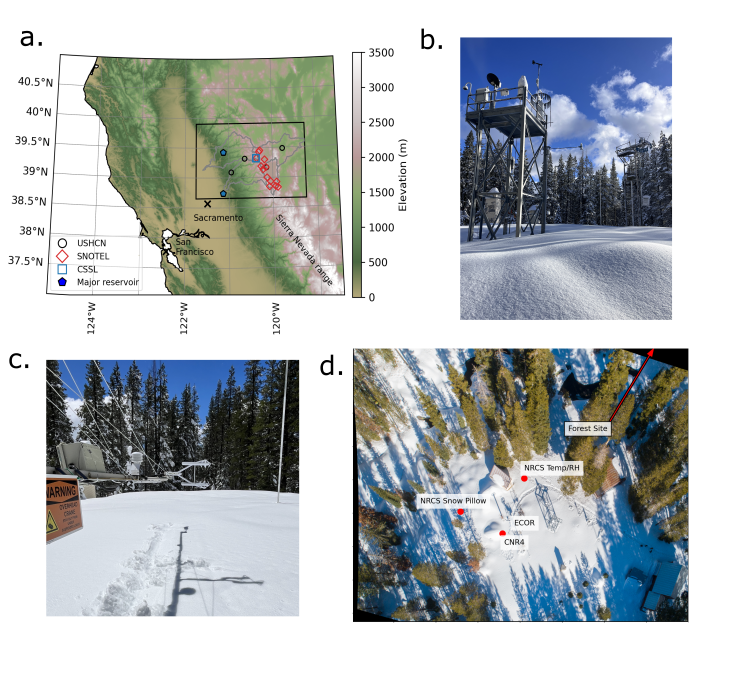
\includegraphics[width=\linewidth]{images2/drawing-1.png}
  \caption{(a) The northern California Sierra Nevada study region with terrain elevation.
  Outlines depict the Yuba, North Fork American, Lake Tahoe, and Truckee HUC8 watershed boundaries.
  Red open diamonds depict the location of NRCS SNOTEL sites, open black circles show the location of the four USHCRN stations in the region, and the open blue square depicts the CSSL energy balance site.
  (b) The CSSL meteorological tower in winter, (c) a close-up view of the Campbell CNR4 radiometer and IRGASON eddy covariance system, and (d) an aerial overview of the CSSL site. The location of the forest meteorological tower (not shown) is located just outside of the frame.
  }
  \label{fig:region_map}
\end{figure}


% USHCRN data
\begin{figure}[htbp]
  \centering
  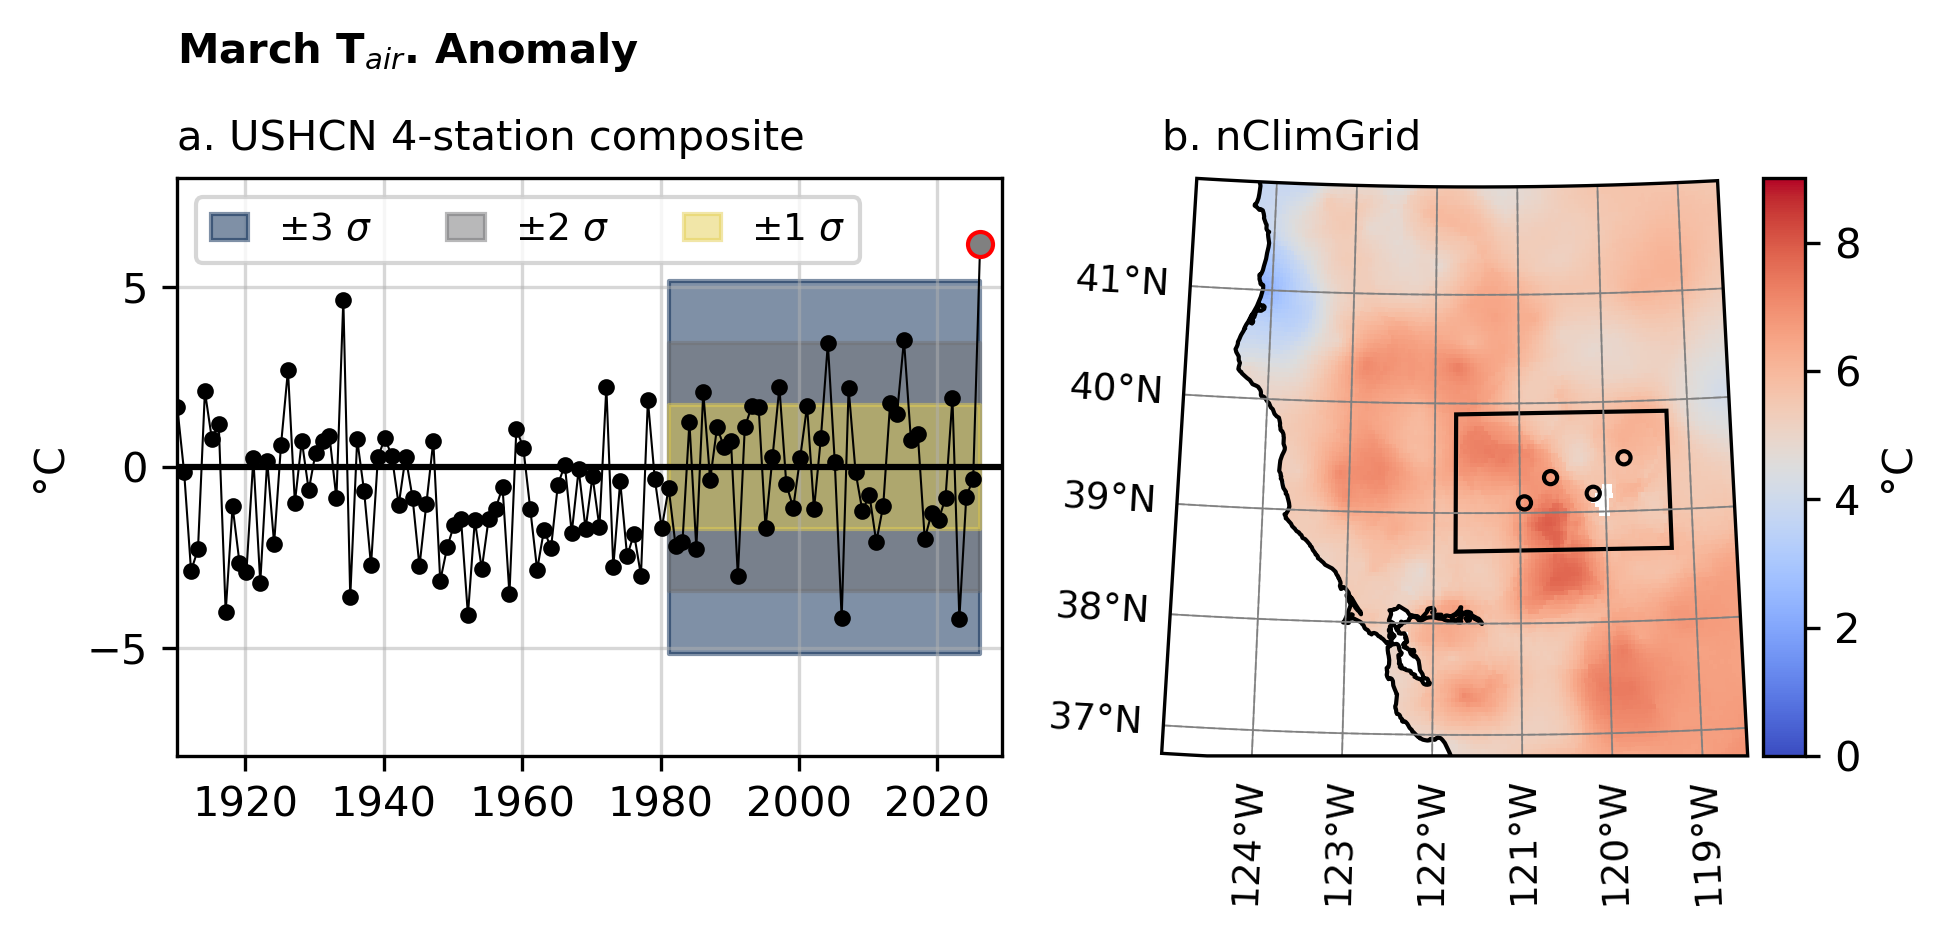
\includegraphics{images2/temp_anomaly_map.png}
  \caption{(a) Composite \tair anomalies from the four HCNv2 dataset stations in the greater Tahoe region study area for the month of March, from 1890 to 2026. Deviations from the 1980--2026 mean are depicted for one, two, and three standard deviation regions (shading).
  Anomalies are computed with respect to the 1981--2010 mean \tair.
  (b) The same, but for a map-view of the \tair anomaly of the gridded nClimGrid product.}
  \label{fig:ushcn_data}
\end{figure}


% ERA5 data
\begin{figure}[htbp]
  \centering
  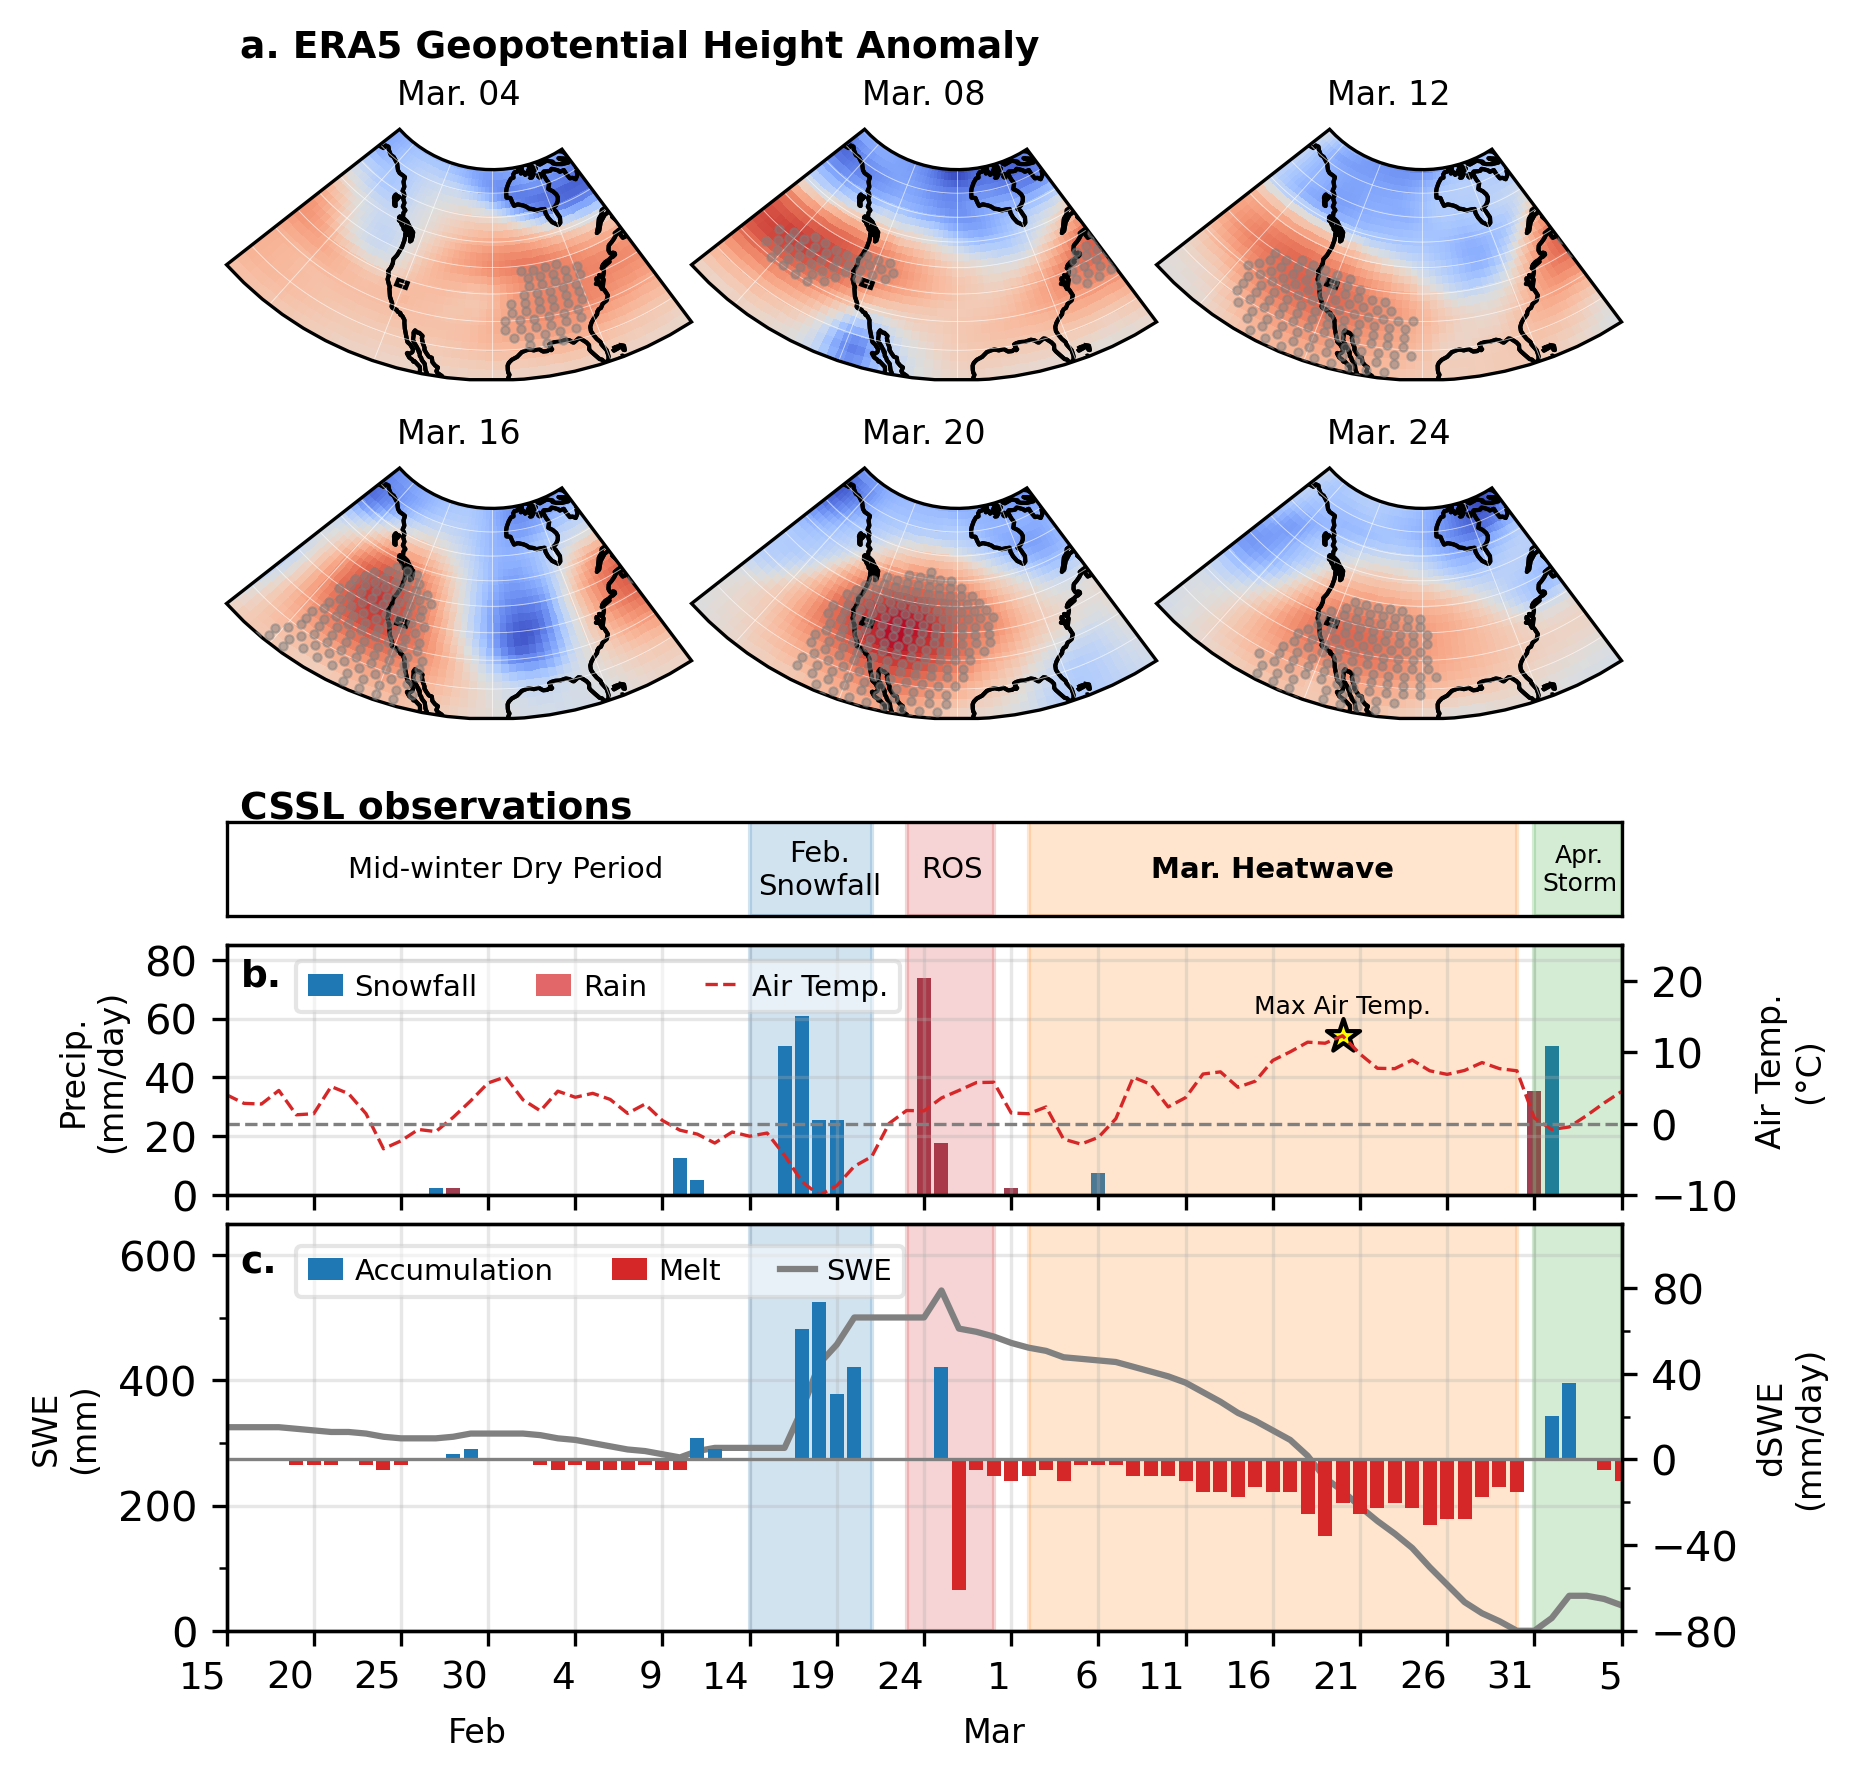
\includegraphics[width=\linewidth]{images2/mar2026_era5_snotel_summary.png}
  \caption{
  (a) The 500 hPa geopotential height anomaly during March 2026 heatwave from ERA5 across the WUS for six individual days.
  The study region is outlined using an overlain black rectangle.
  Gray stippling indicates regions with 500 hPa geopotential height anomalies greater than 2-$\sigma$ above the 1981--2010 mean for the month of March.
  (b) depicts two meter \tair anomaly z-scores from the Tahoe City COOP station. 
  Periods meeting the \cite{Rhoades2026-jm} SEHW criteria are outlined with a black box. 
  (c) shows the time series of meteorological and snow conditions at CSSL, with different synoptic conditions highlighted by background shading (top-panel).
  Wind speed, precipitation with rain and snow differentiated, and two-meter \tair are depicted.
  The bottom panel depicts modeled (SUMMA) and observed SWE at the open and forest sites. 
  Average rates of SWE loss are listed in the figure text with dashed lines superimposed on the SWE curves.
  }
  \label{fig:era5_anoms}
\end{figure}


\begin{figure}[htbp]
  \centering
  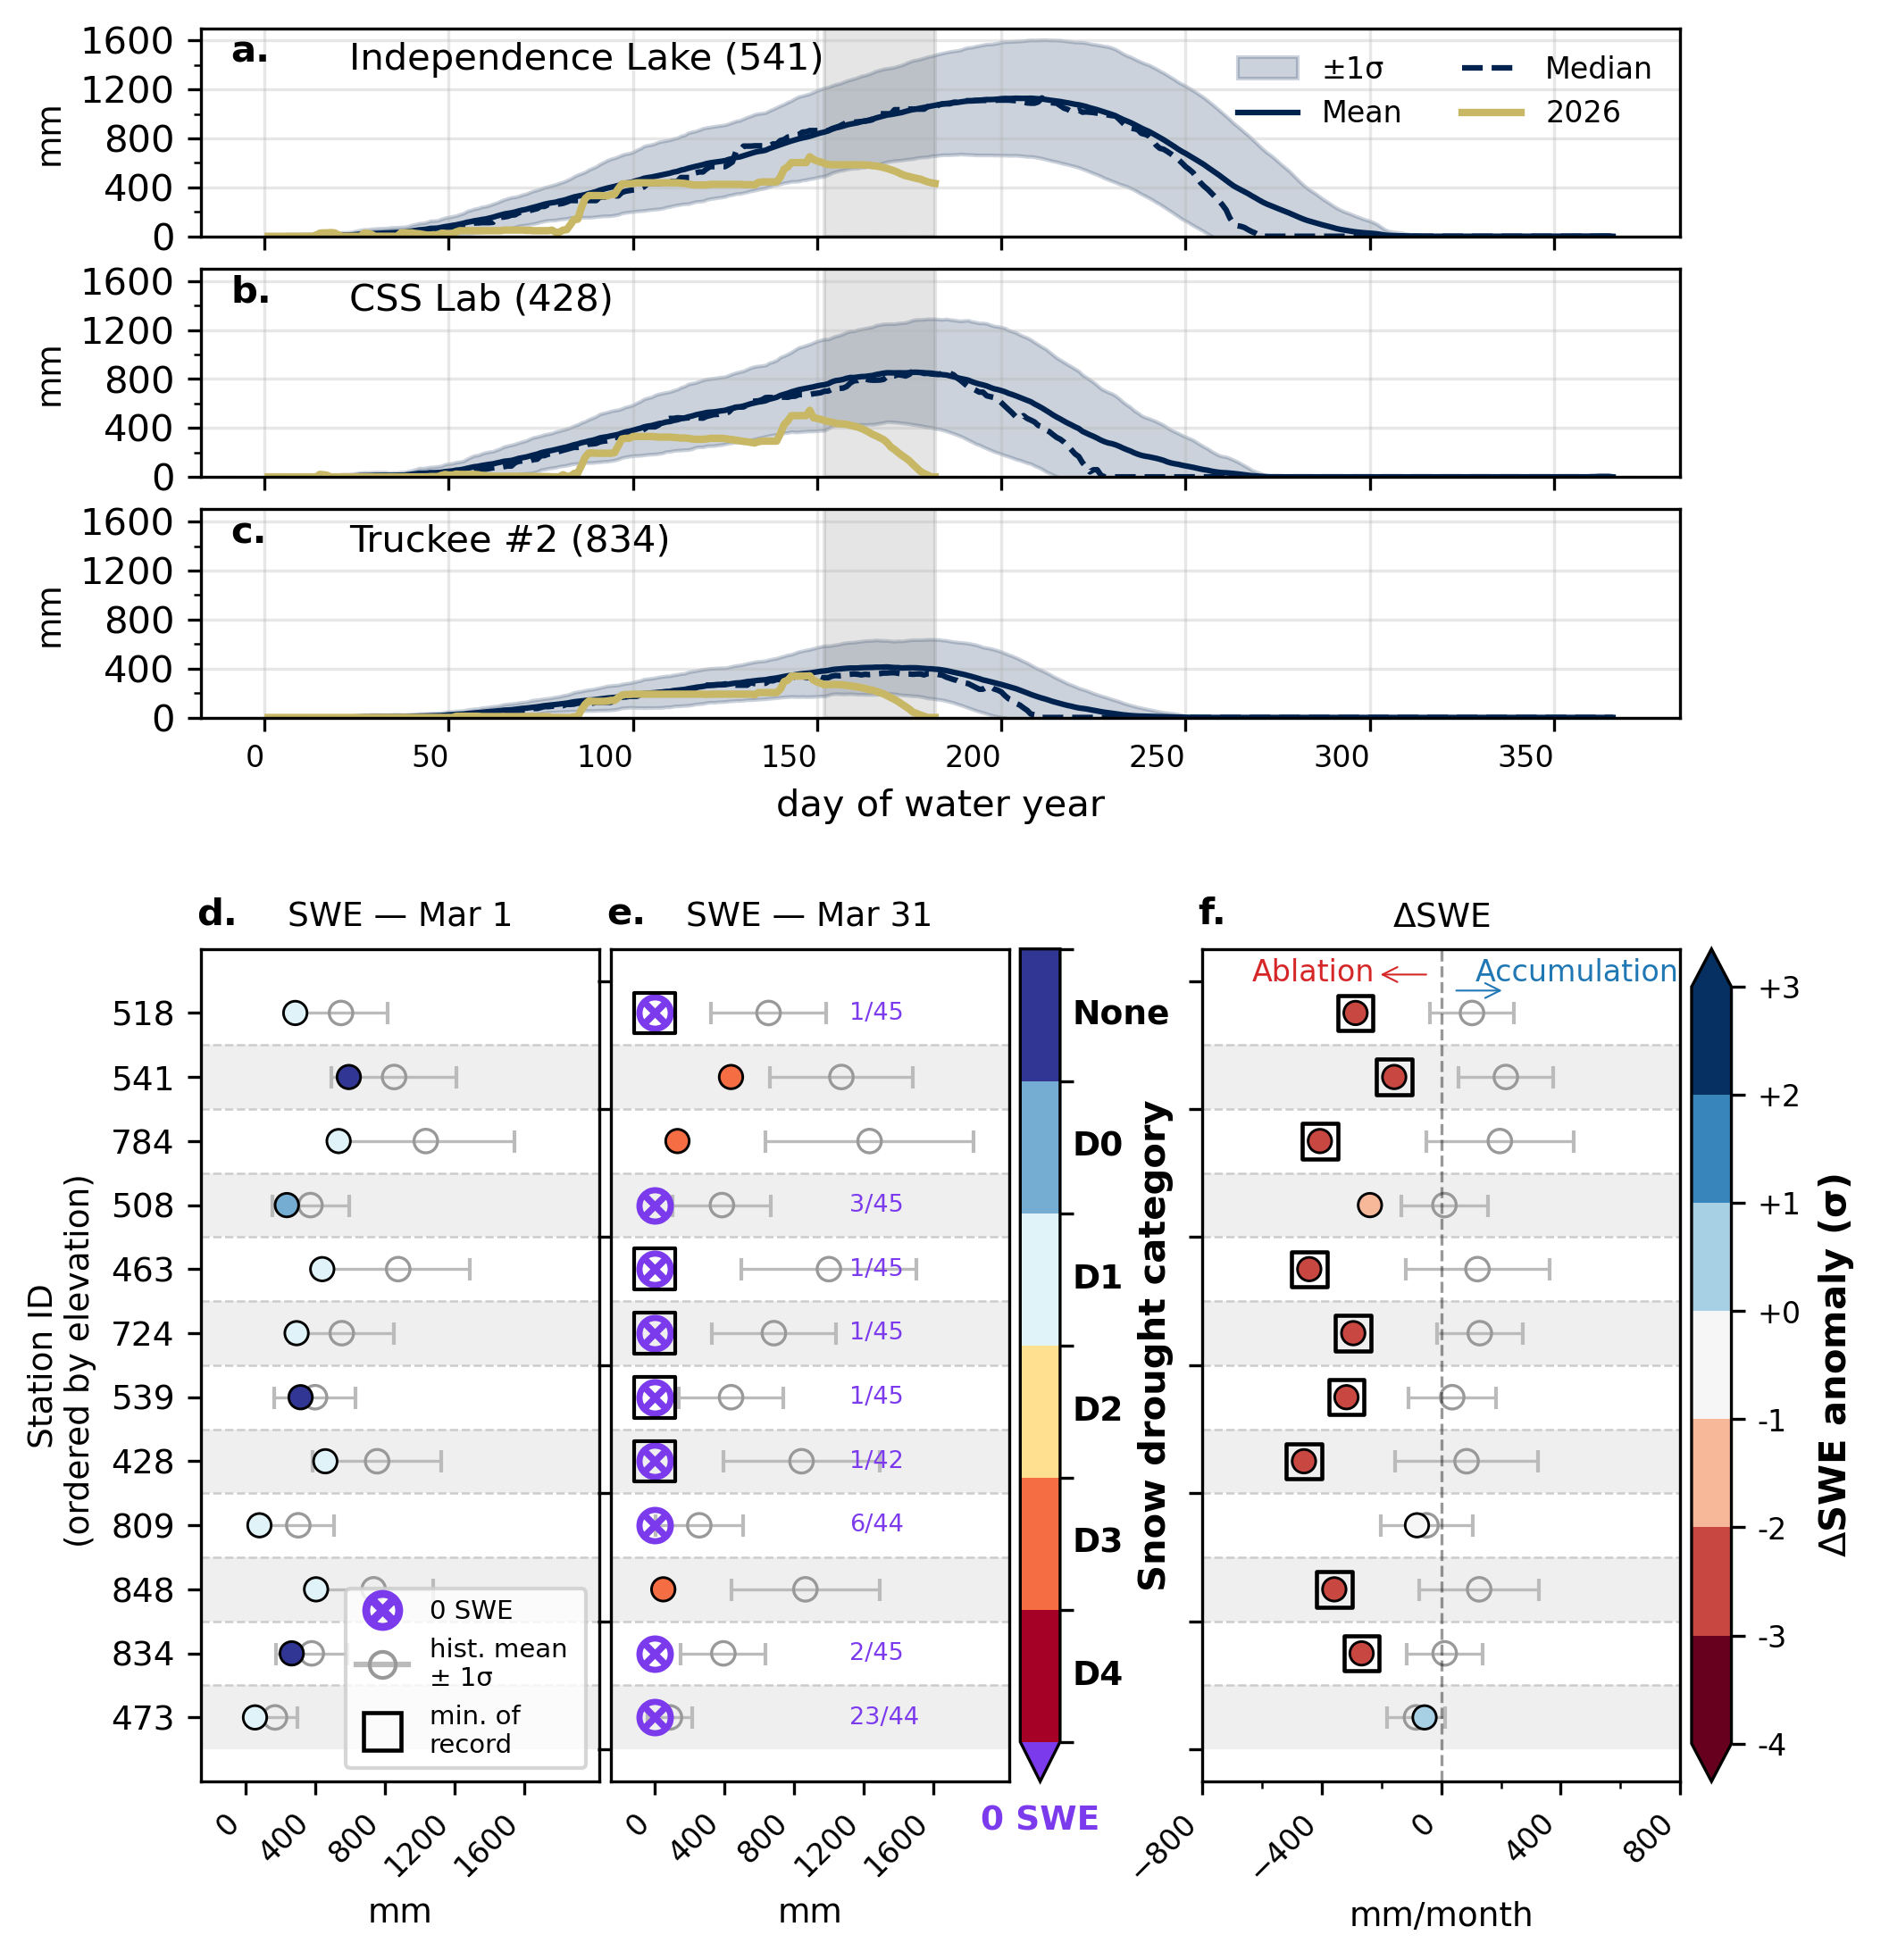
\includegraphics[width=\linewidth]{images2/swe_change_2026_v2.png}
  \caption{(a--c) A timeseries of SWE at three SNOTEL stations in the study region.
  The mean, median (dashed line), 1 standard-deviation (shaded region) and water year 2026 values are depicted.
  (d) SWE values on March 1st for the 12 SNOTEL sites in the study domain, labeled by their three-digit station code.
  (e) The same as (d), but for SWE on March 31.
  Color values correspond with the snow drought D-scale.
  A 0 mm of SWE value is depicted by a purple circle marker.
  The purple text lists the number of 0 mm SWE occurrences observed on that date relative to the period of record for that site.
  (f) The SWE change between Mar 31 and Mar 1 (mSWE) compared with the historical record.
  Color values depict the deviation from the mean in units of standard deviation.
  Square markers bounding symbols indicate that the SWE or mSWE is the record minimum for the period of record.
  }
\label{fig:swechange}
\end{figure}


% \begin{figure}[htbp]
%   \centering
%   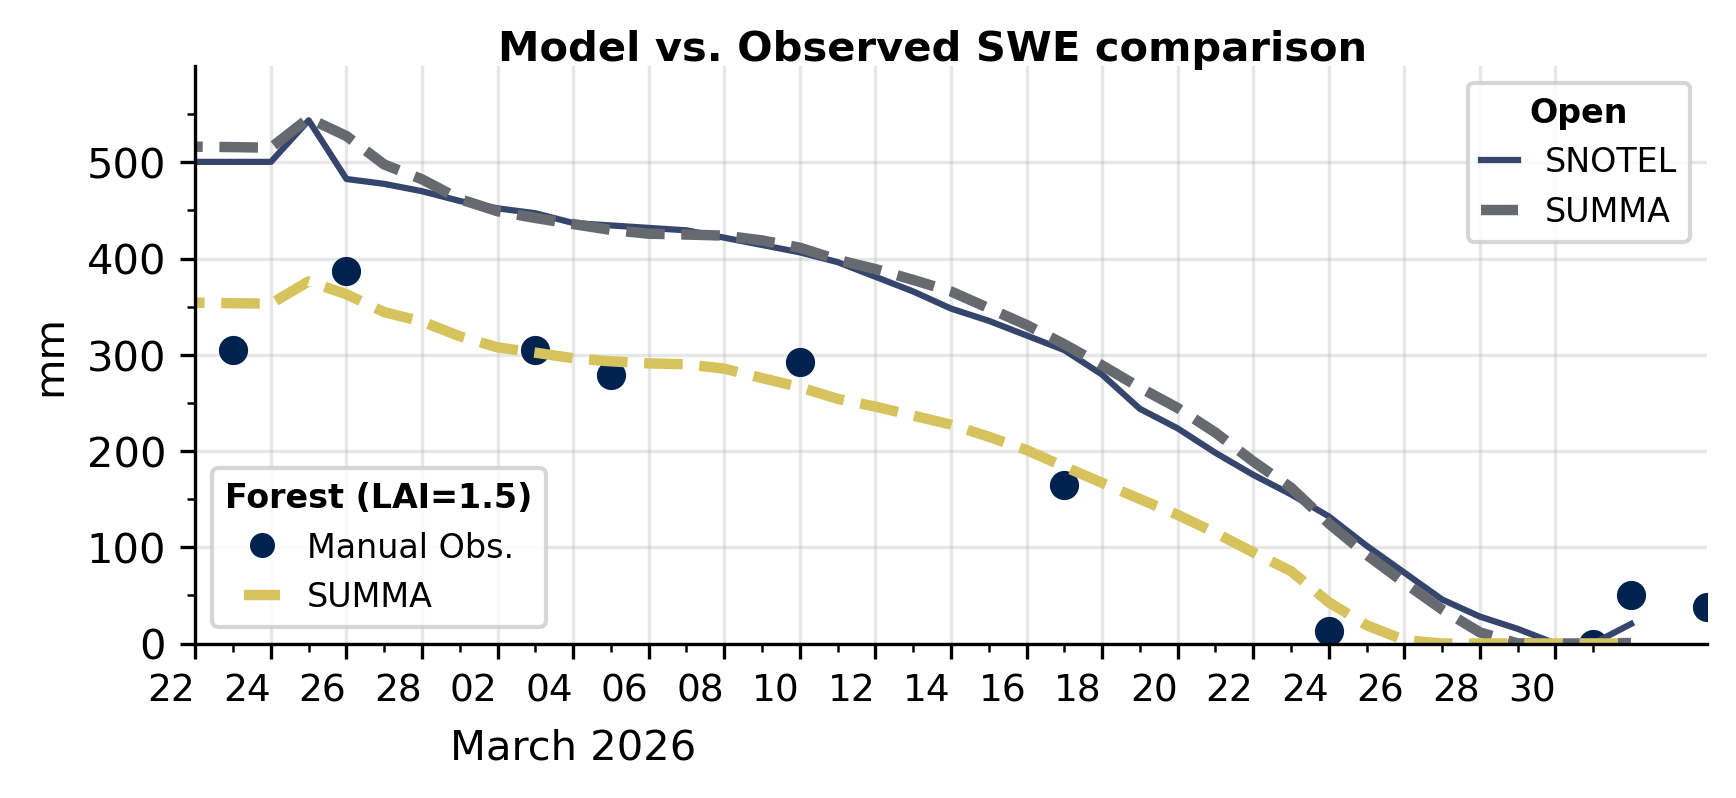
\includegraphics{images2/SWE_forest_v_open.png}
%   \caption{\todo{highlight the time range that is displayed in the next two figures}. A comparison of daily SWE in the open (NRCS snow pillow) and forest (manual federal sampler measurements) against the SUMMA model (dashed gray and yellow lines, respectively).}
%   \label{fig:forest_v_open_swe}
% \end{figure}


\begin{figure}[htbp]
  \centering
  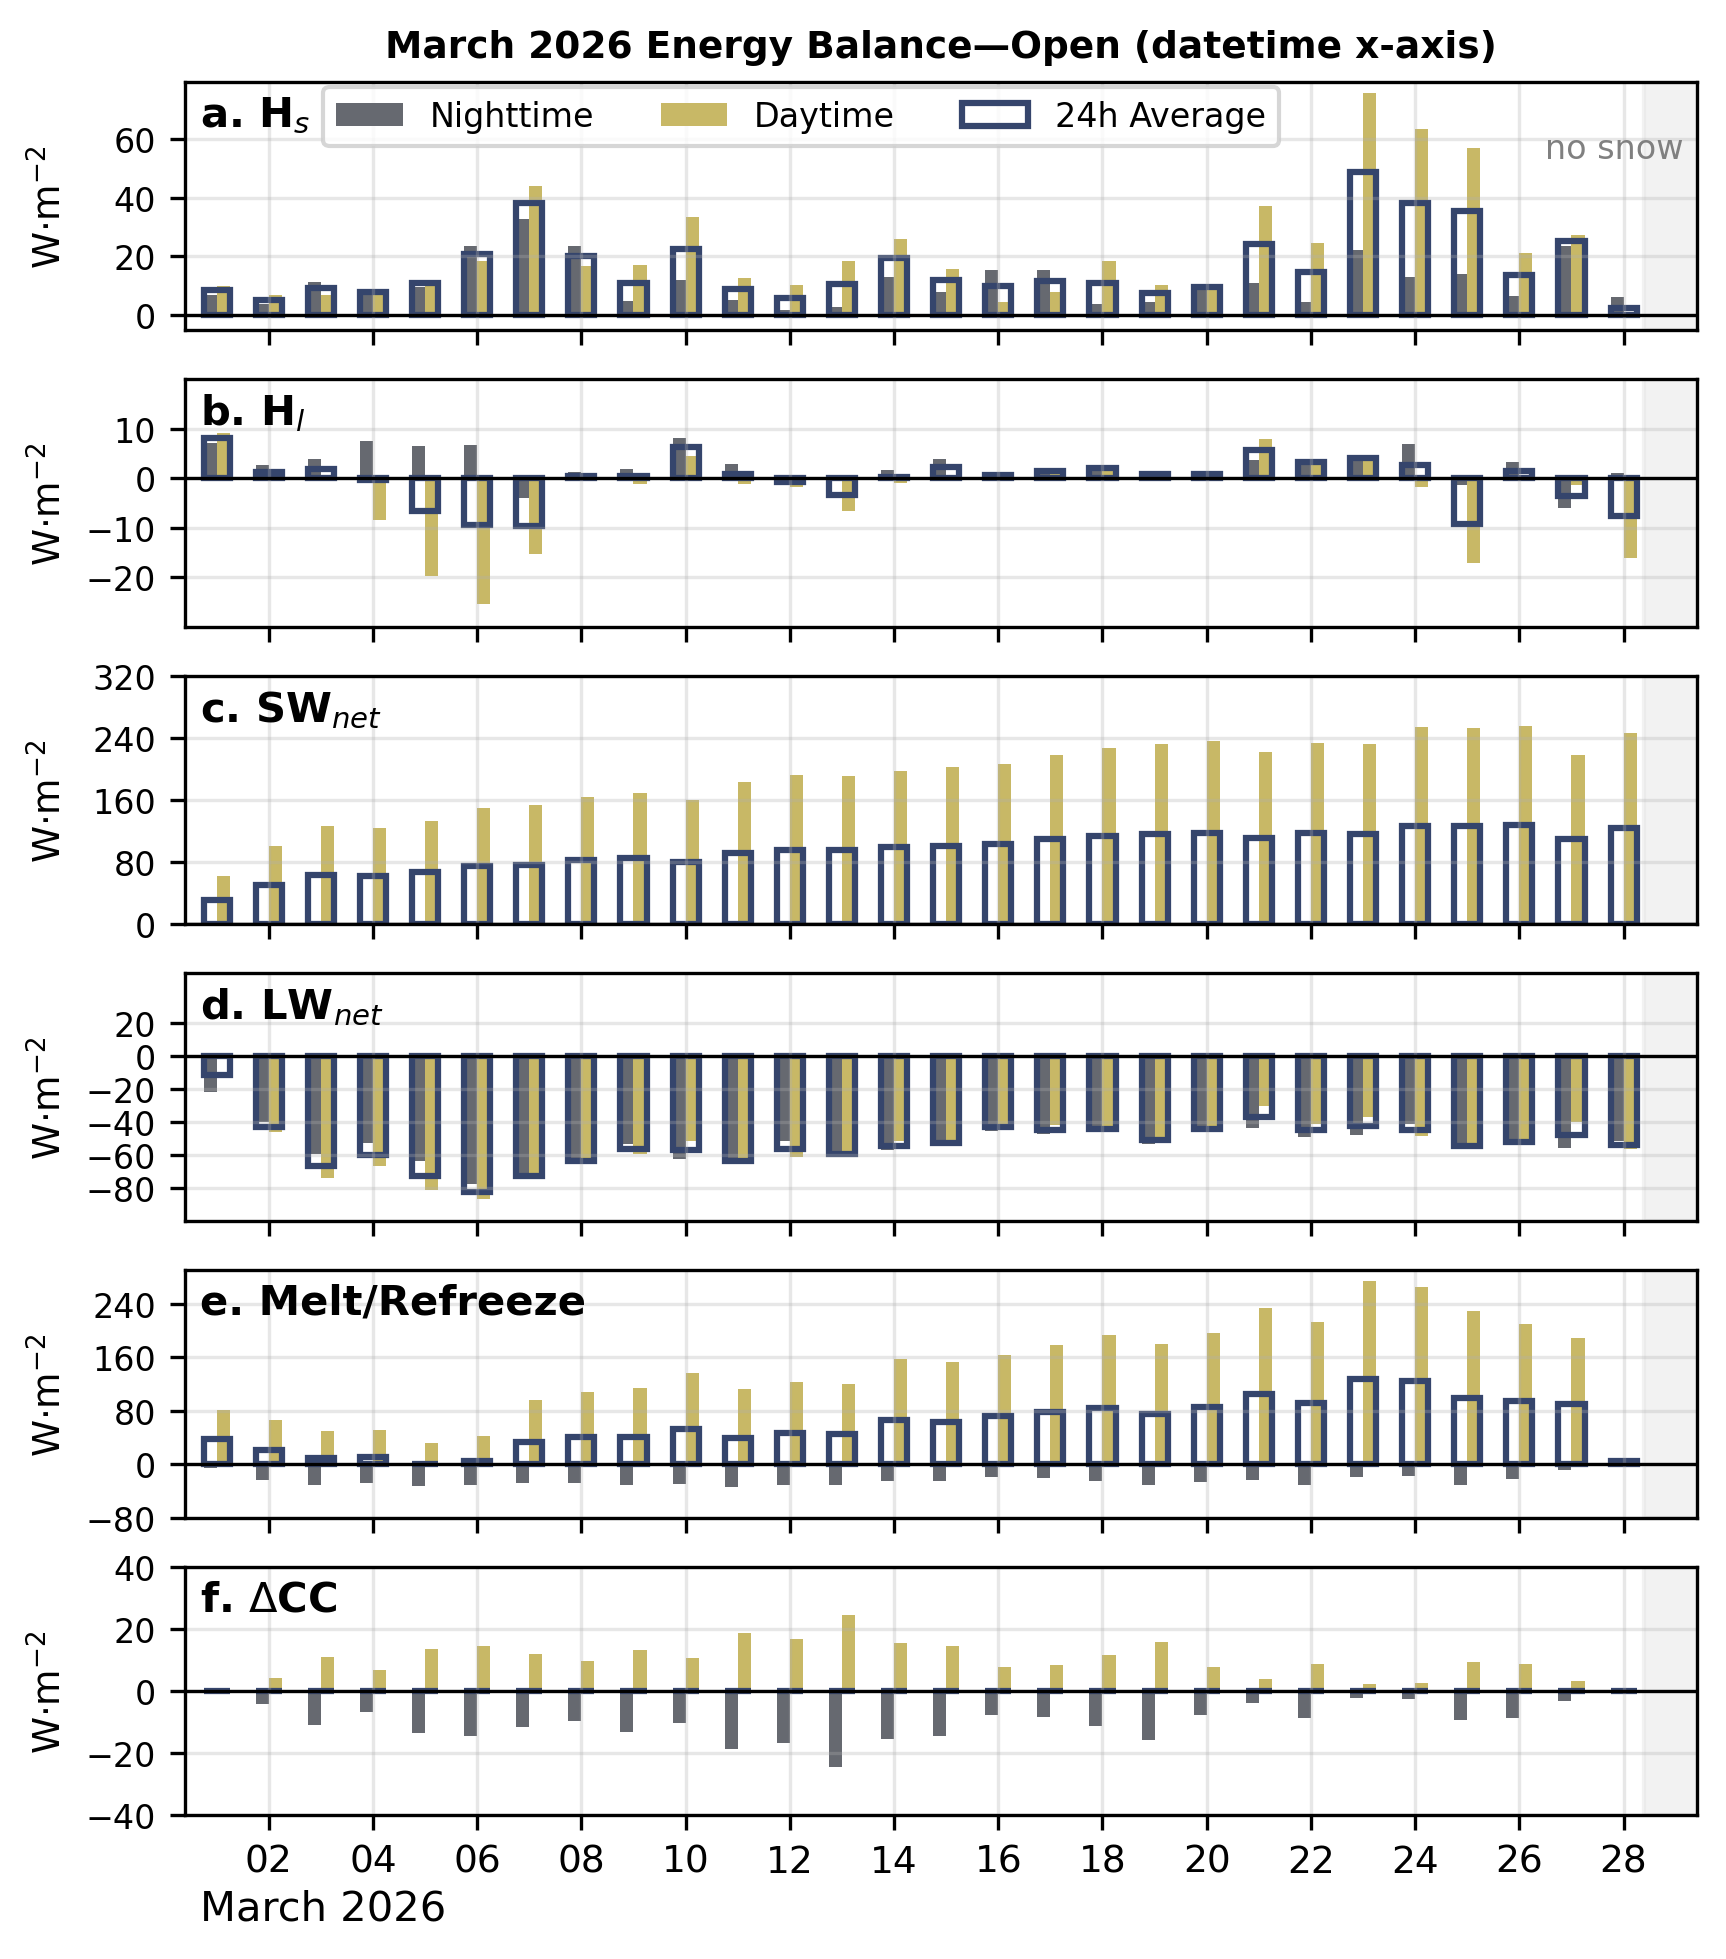
\includegraphics[width=\linewidth]{images2/mar_seb_open.png}
  \caption{Daily average energy flux components including (a) $H_s$, (b) $H_l$, (c) \swnet, (d) \lwnet, (e) snowpack Melt/Refreeze and (f) change in cold-content ($\Delta$ CC) during the March 2026 heatwave at the open site.
  Each day has three bars: the left-most yellow bar depicts the daytime flux, the right-most gray bar depicts the nighttime flux, and the outline spanning both bars depicts the 24-hour average flux.
  Please note that the y-scales are not equivalent across all of the figures.
  }
  \label{fig:open_seb}
\end{figure}



\begin{figure}[htbp]
  \centering
  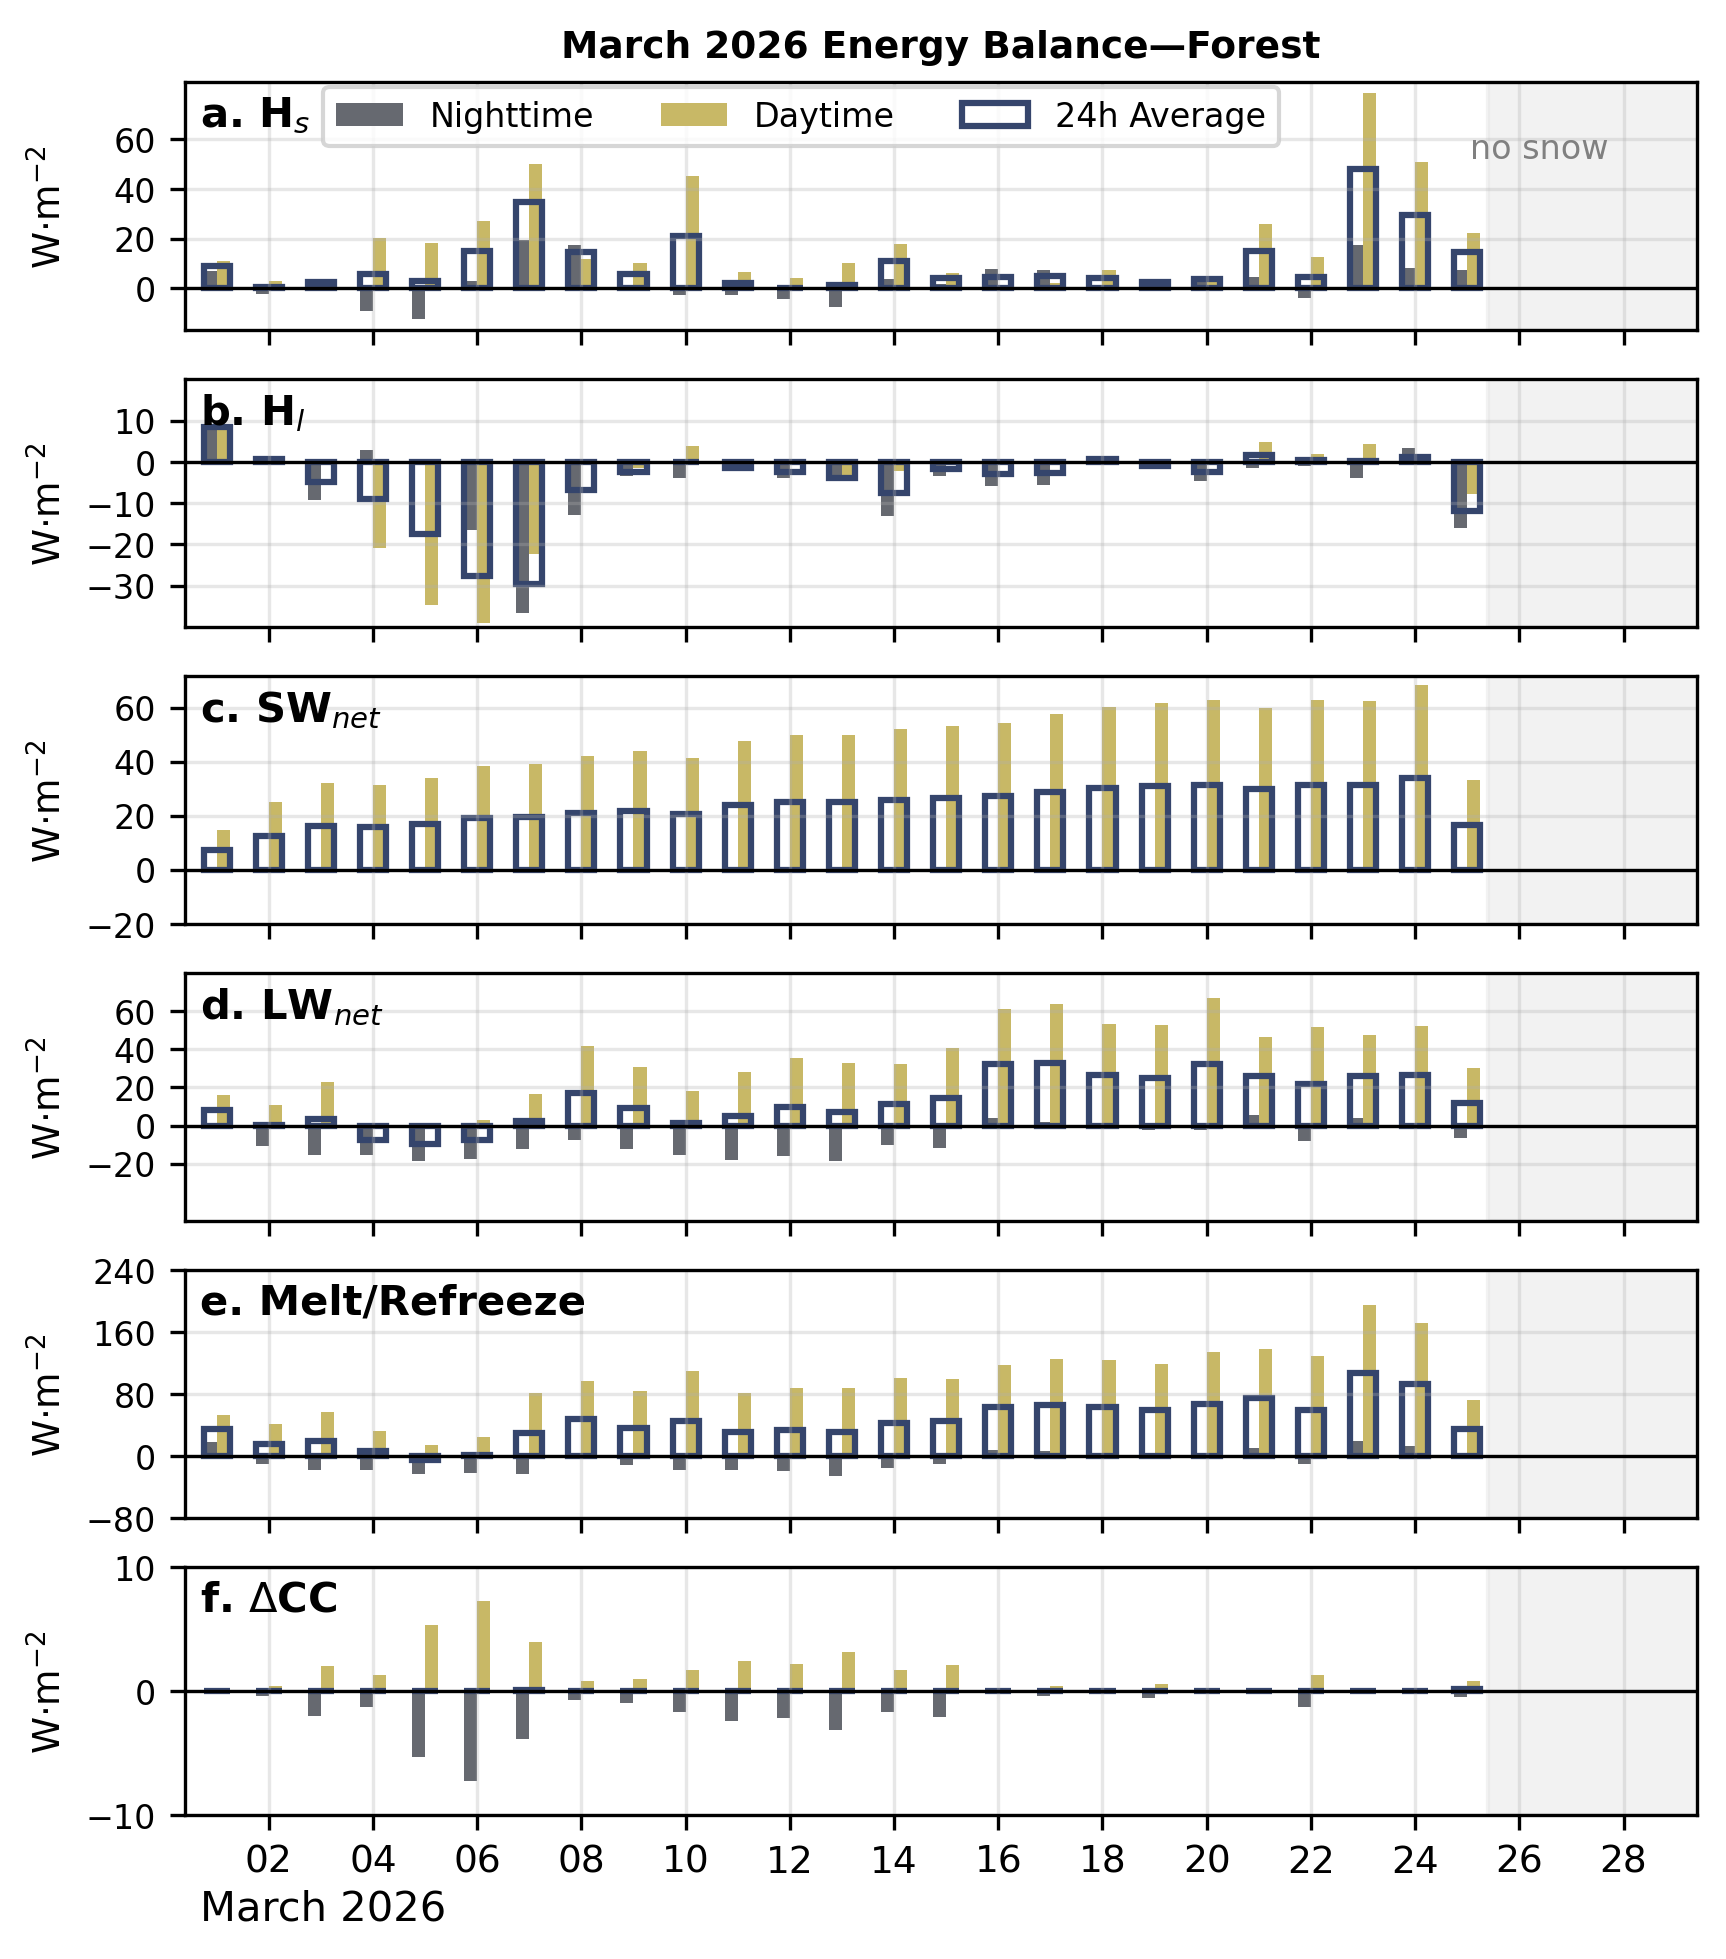
\includegraphics[width=\linewidth]{images2/lai_p5_seb.png}
  \caption{The same as \fignop{fig:open_seb}{} but for the forest site.
   Note that the y-axis limits and ticks are not the same as in that figure.}
  \label{fig:forest_seb}
\end{figure}


\begin{figure}[htbp]
  \centering
  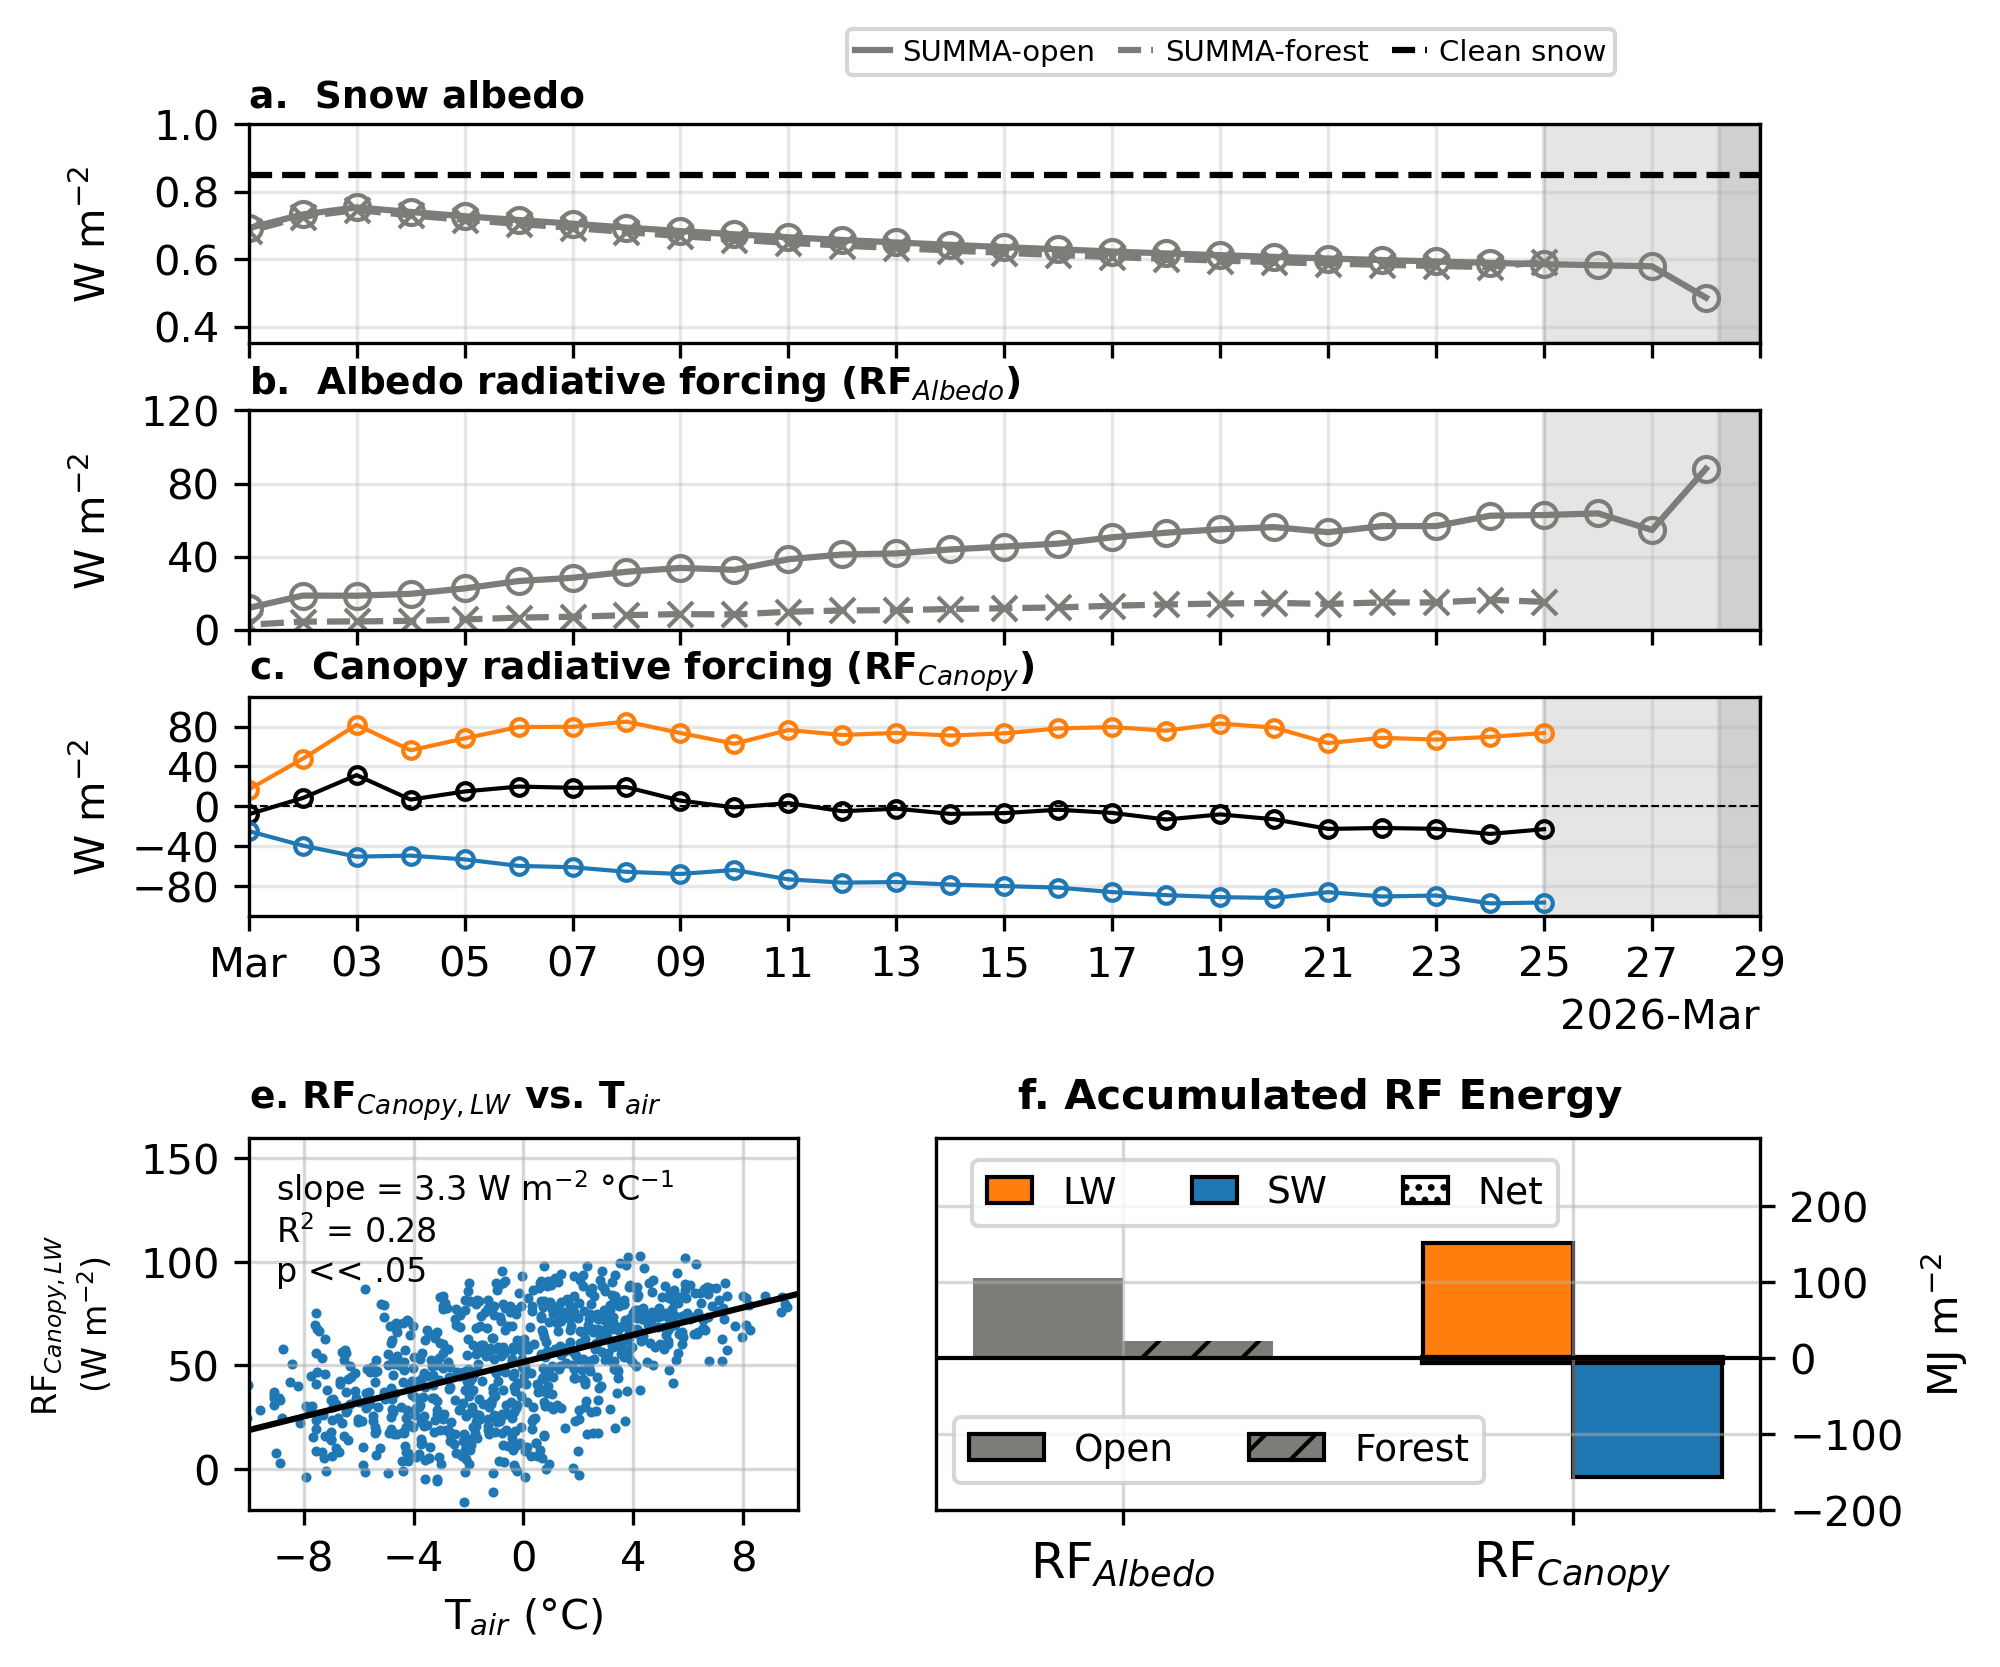
\includegraphics[width=\linewidth]{images2/canopy_lw_radiation_effect_and_albedo.png}
  \caption{Timeseries of (a) \albedo, (b) \rfalb, (c) \rfcanopy, (d) \rfcirrus for March 2026. 
  LW and SW components are depicted in (c) and (d).
  Net (LW + SW) components are also depicted in (c).
  (e) depicts the relationship between daily-average \tair and the LW component of \rfcanopy for all Marches in the SUMMA historical record (2000--2026).
  (f) depicts accumulated energy terms during the snow-covered duration of March.
  }

  \label{fig:radiative_forcing}
\end{figure}


\begin{figure}[htbp]
  \centering
  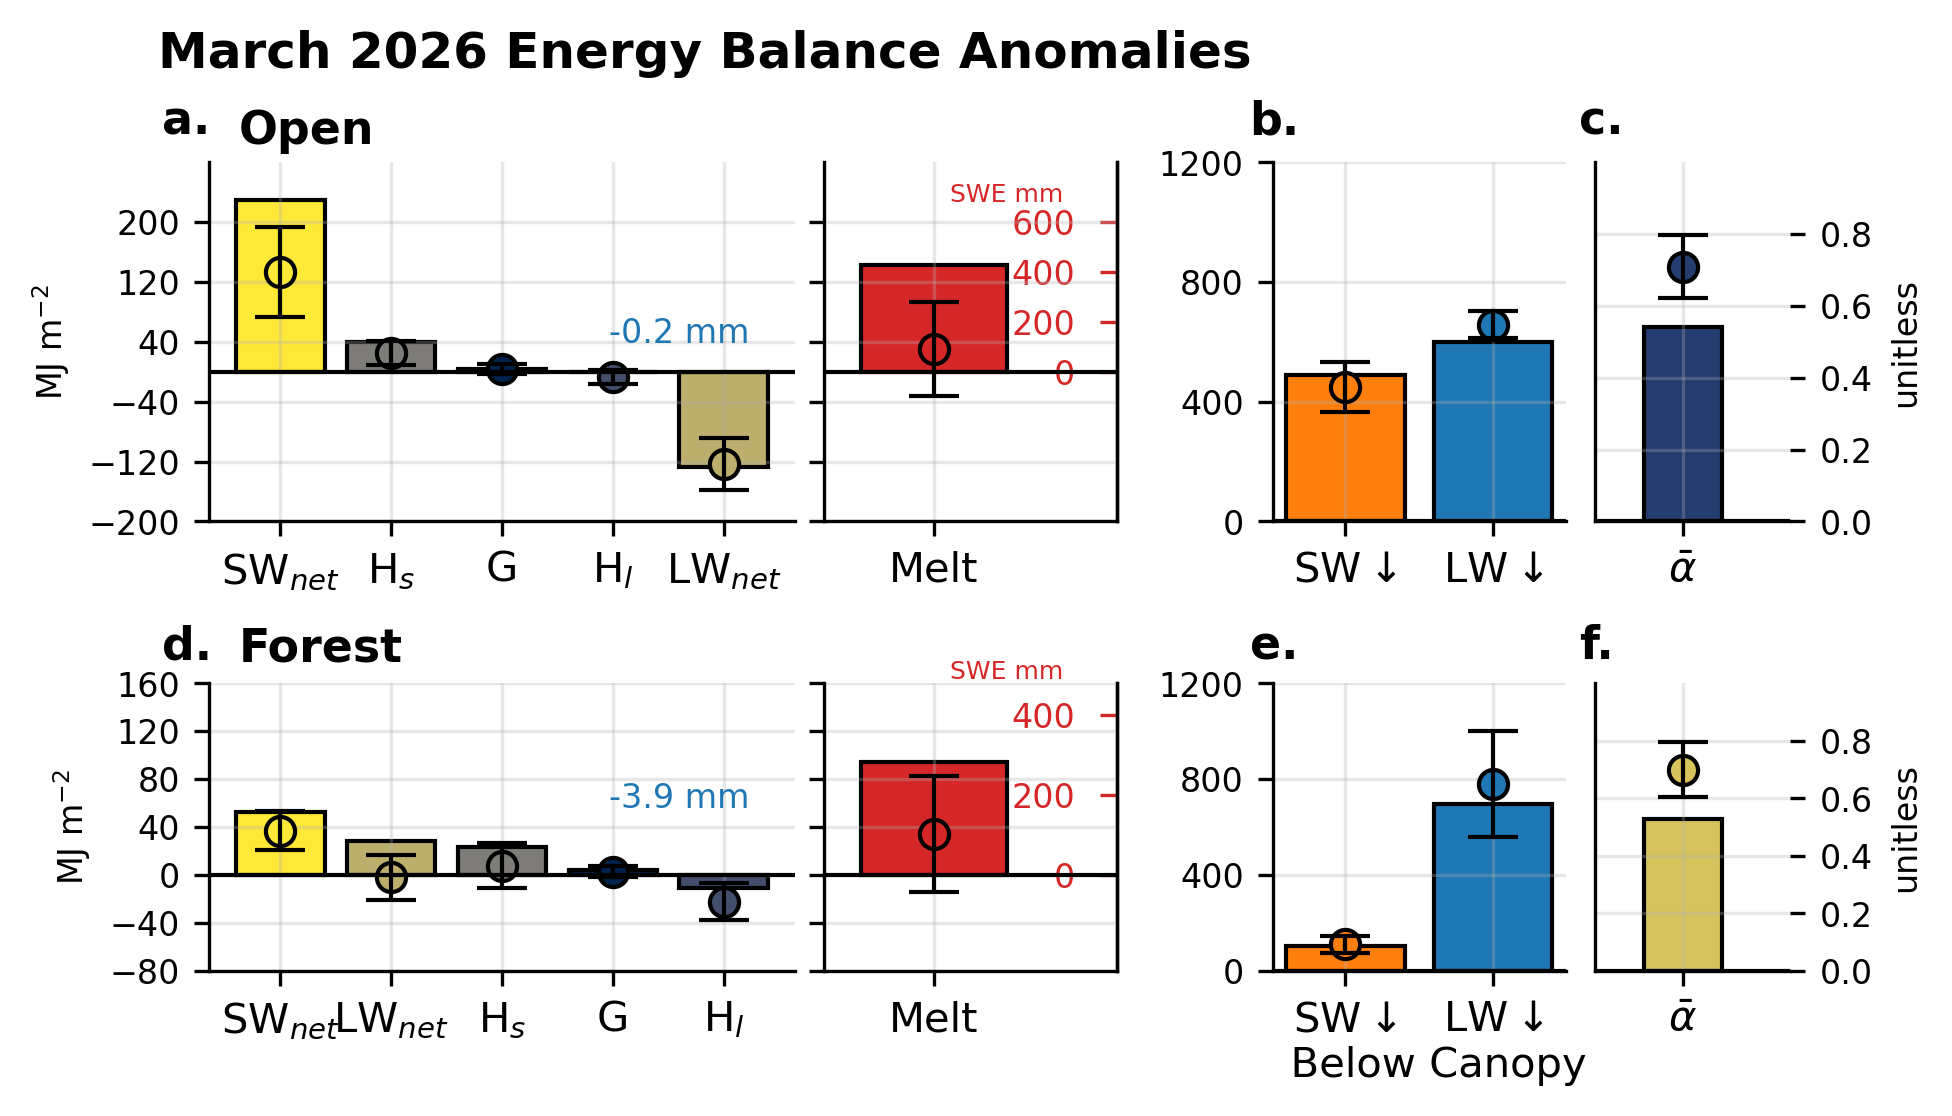
\includegraphics{images2/mar_seb_open_v_forest.png}
\caption{Accumulated snow energy fluxes (\swnet, \lwnet, \hs, \hlat, G), Melt, radiation forcings,
(\swdn, \lwdn), and weighted snow $\bar{\alpha}$ for the open (a--c) and forest (d--f) sites for the duration of March, restricted to times when SWE is present.
Open circles and whiskers show the averages and one-standard deviation from the March SUMMA historical period (2000--2026).
Equivalent units of mm of melt are displayed in red text on the right-hand side of the Melt panel.
The under-canopy \swdn and \lwdn are depicted in panel (e).
}\label{fig:monthly_seb_mar}
\end{figure}


\begin{figure}[htbp]
  \centering
  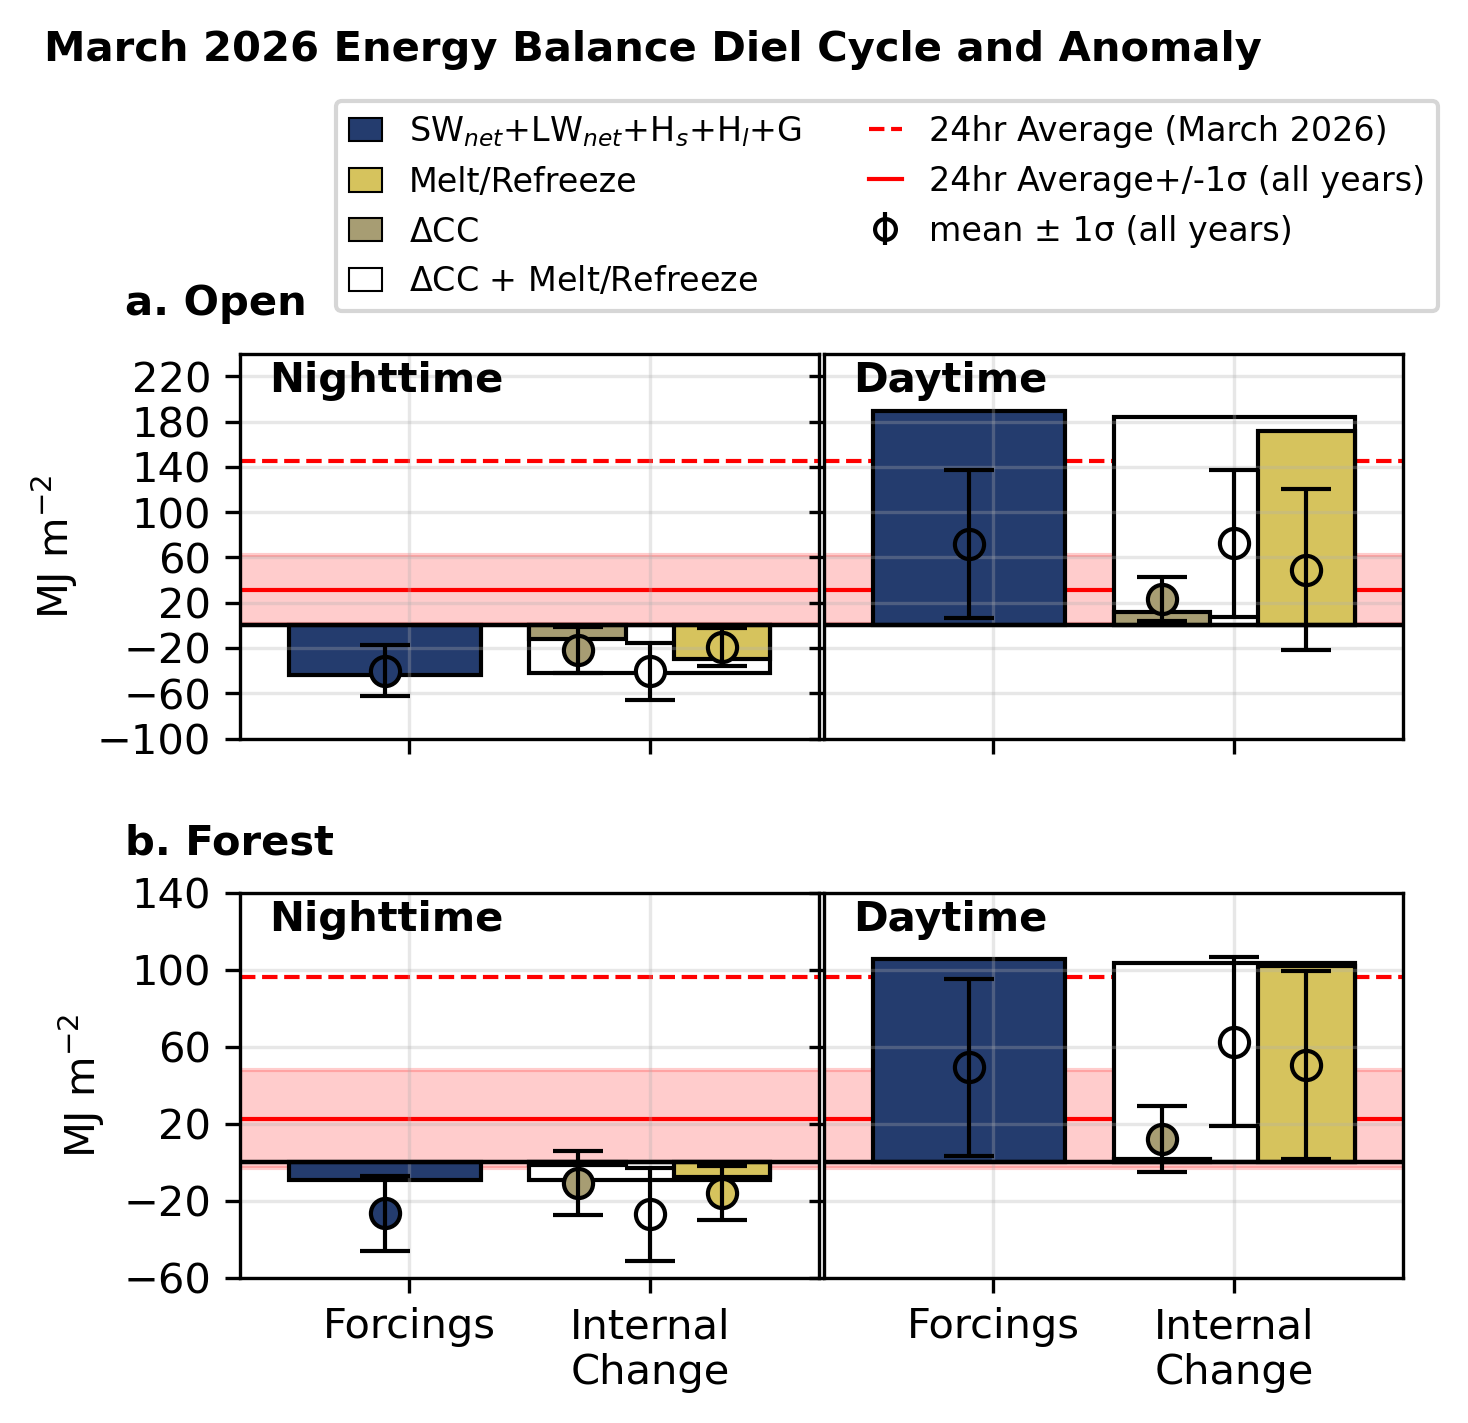
\includegraphics[width=\linewidth]{images2/mar_diel_seb_open_v_forest.png}
  \caption{Similar to Fig. \ref{fig:monthly_seb_mar}, but for daytime, nighttime, and 24hr sums of accumulated energy balance components in the (a) Open and (b) Forest sites.
  Forcings include net-radiative and turbulent flux terms at top and bottom boundaries of the snowpack.
  Internal Change terms are the accumulated change in Cold-Content and Melt (positive) and Refreezing (negative) energy.
  $\Delta$CC and Melt/Refreeze are separated into individual terms for visualization purposes.
  }
  \label{fig:mar_diel_seb_open_v_forest}
\end{figure}


\begin{figure}[htbp]
  \centering
  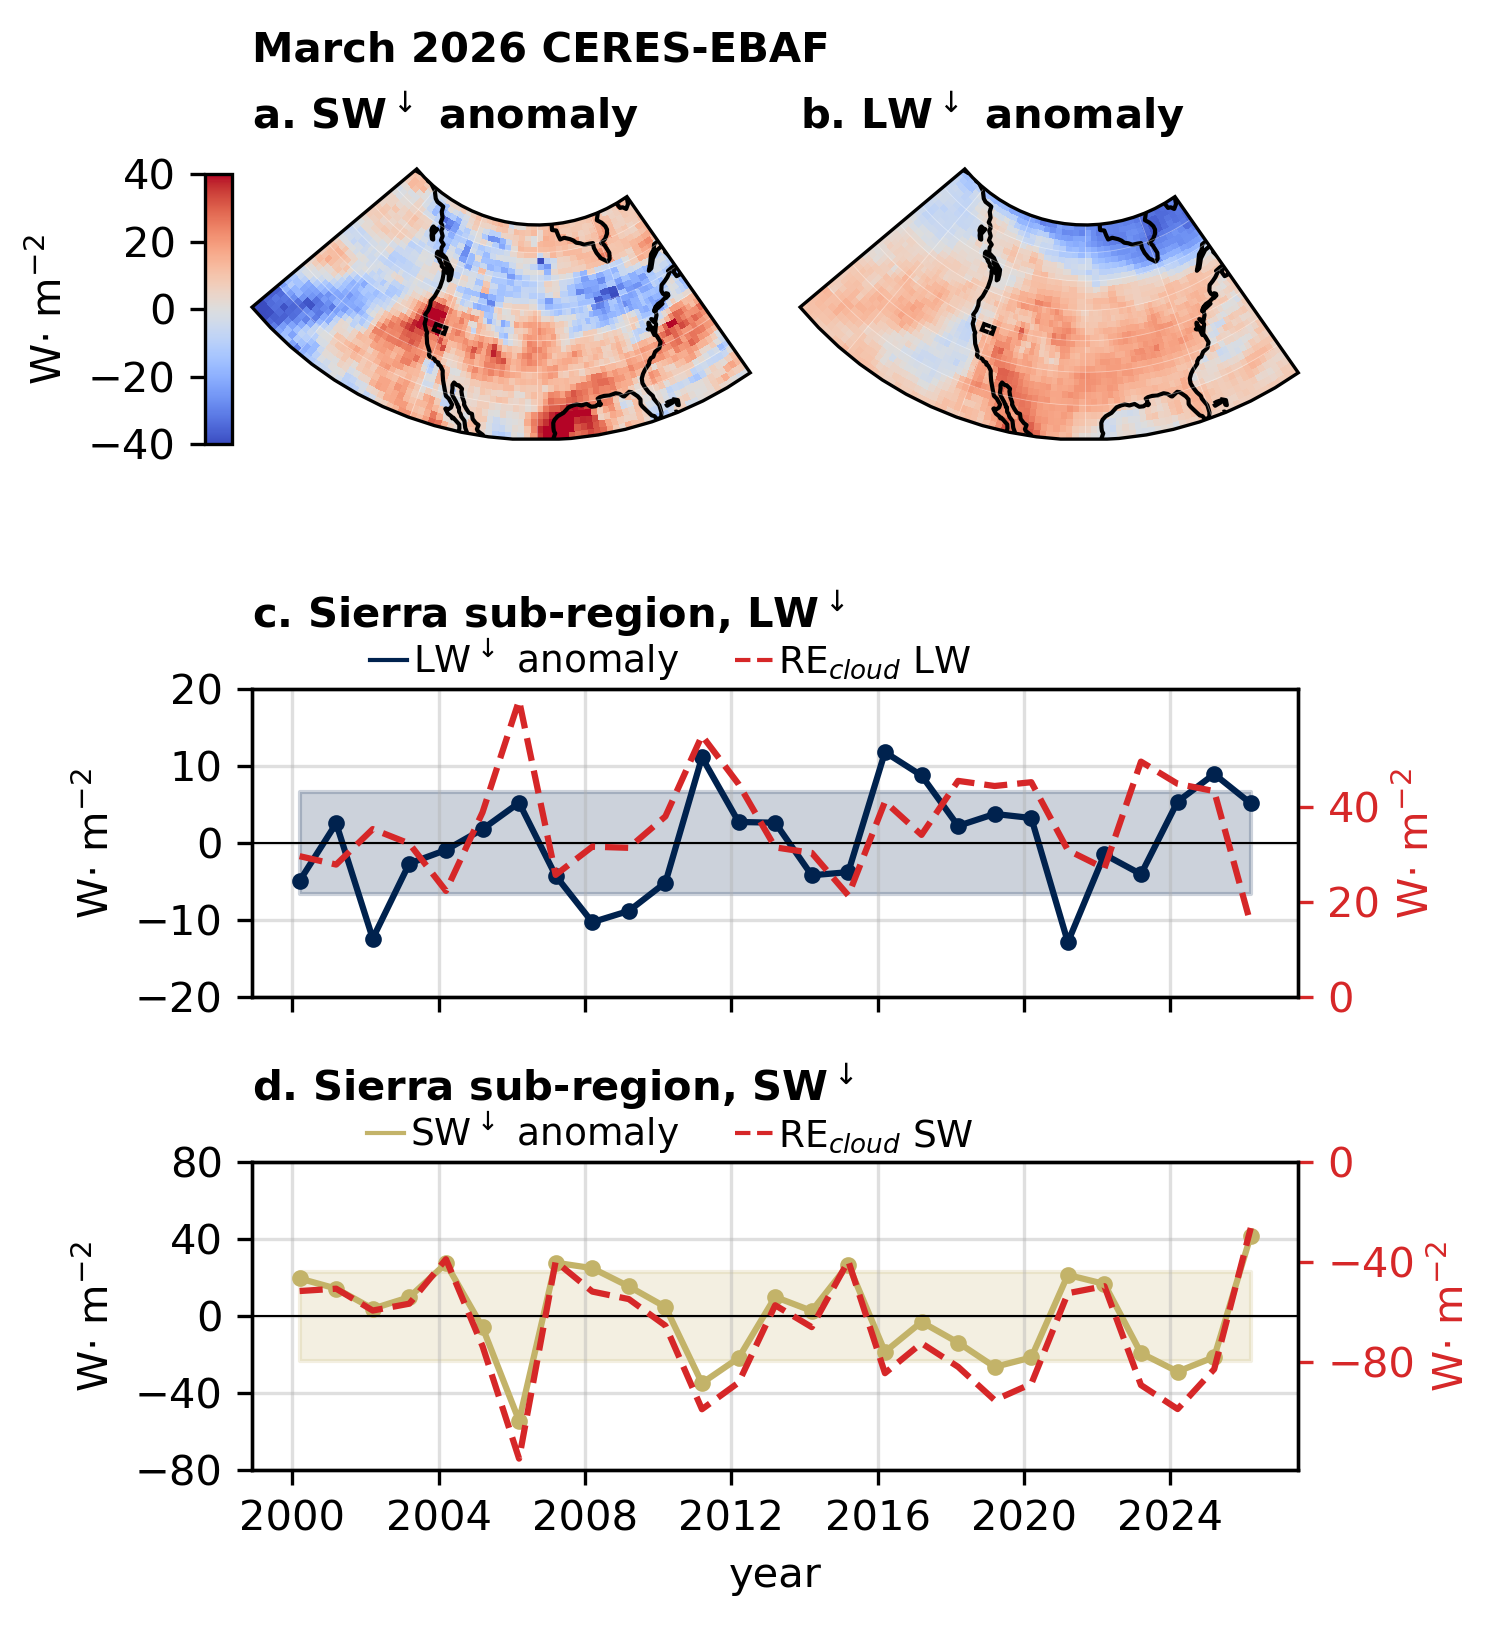
\includegraphics{images2/ceres_ebaf_anomaly.png}
  \caption{March \swdn (a) and \lwdn (b) anomalies (relative to the March 2000 to present record) from the CERES-EBAF 1x1 degree resolution product.
  (c) and (d) depict the timeseries of anomalies averaged over the Sierra Nevada study region.
  RE$_{cloud}$ amount is depicted with a twin y-axis, with units displayed on the right-hand side in red text.
  The shaded region in each plot depicts one standard deviation of the anomaly.
  }
  \label{fig:ebaf_anomaly}
\end{figure}




% \begin{figure}[htbp]
%   \centering
%   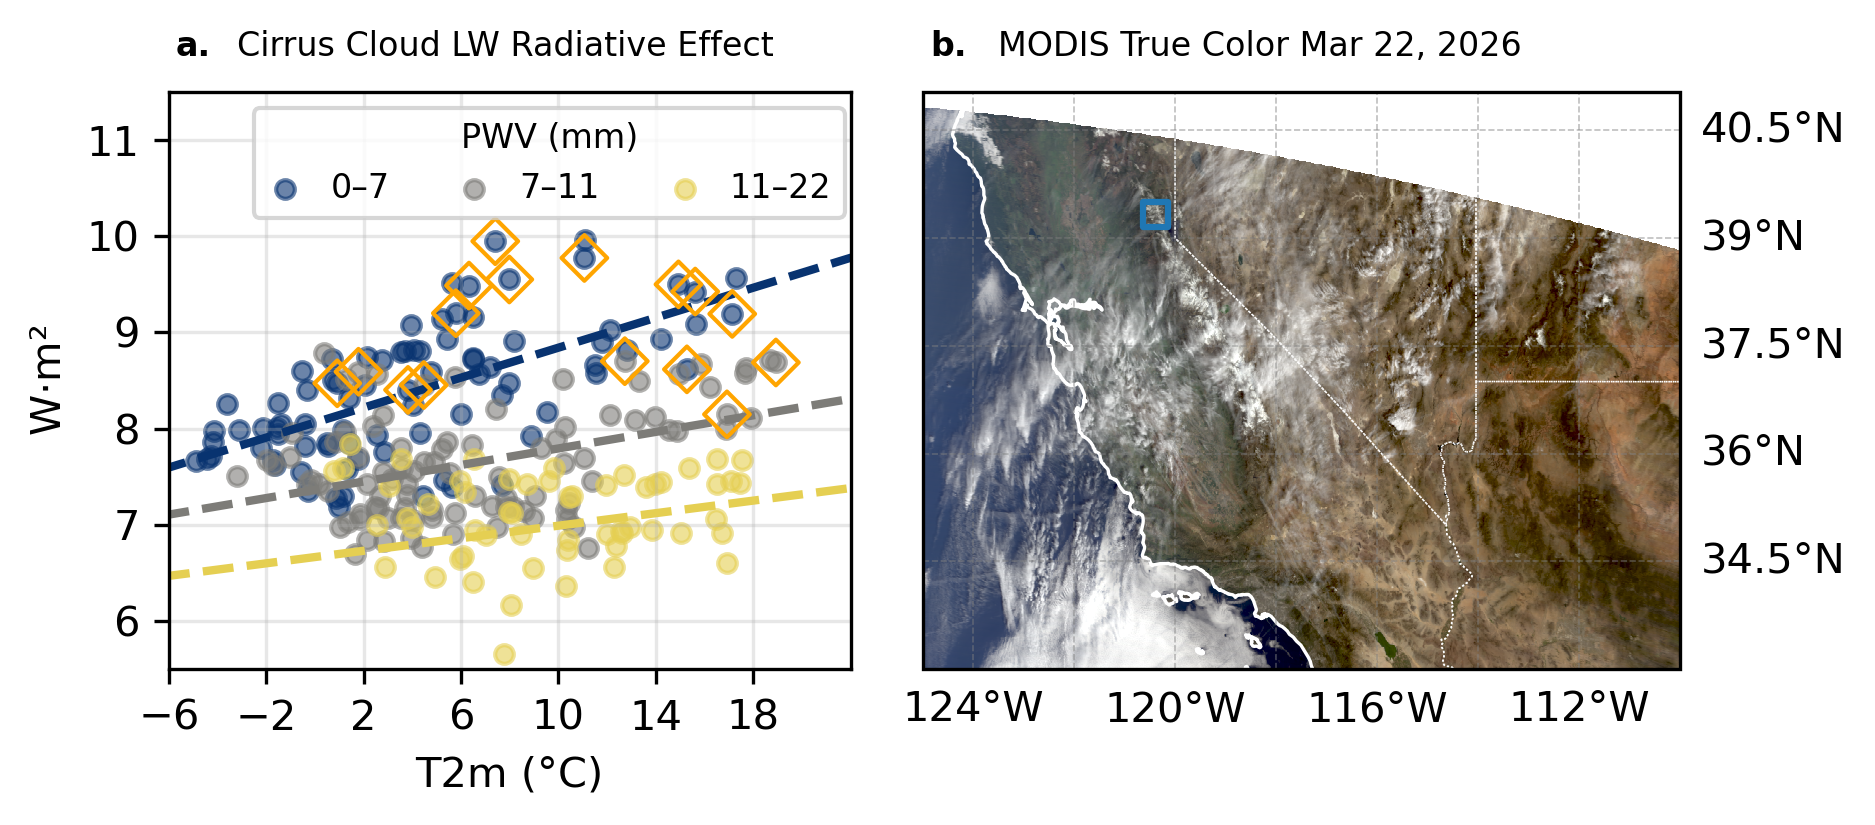
\includegraphics{images2/cirrus_effect.png}
%   \caption{The daily-averaged cCRF$_{Net}$ during March 2026 as simulated by RRTMG for the surface (cCRF$_{Net, sfc}$) and top-of-atmosphere (cCRF$_{Net, TOA}$).
%   }
%   \label{fig:cirrus_longwave}
% \end{figure}


% \begin{figure}[htbp]
%   \centering
%   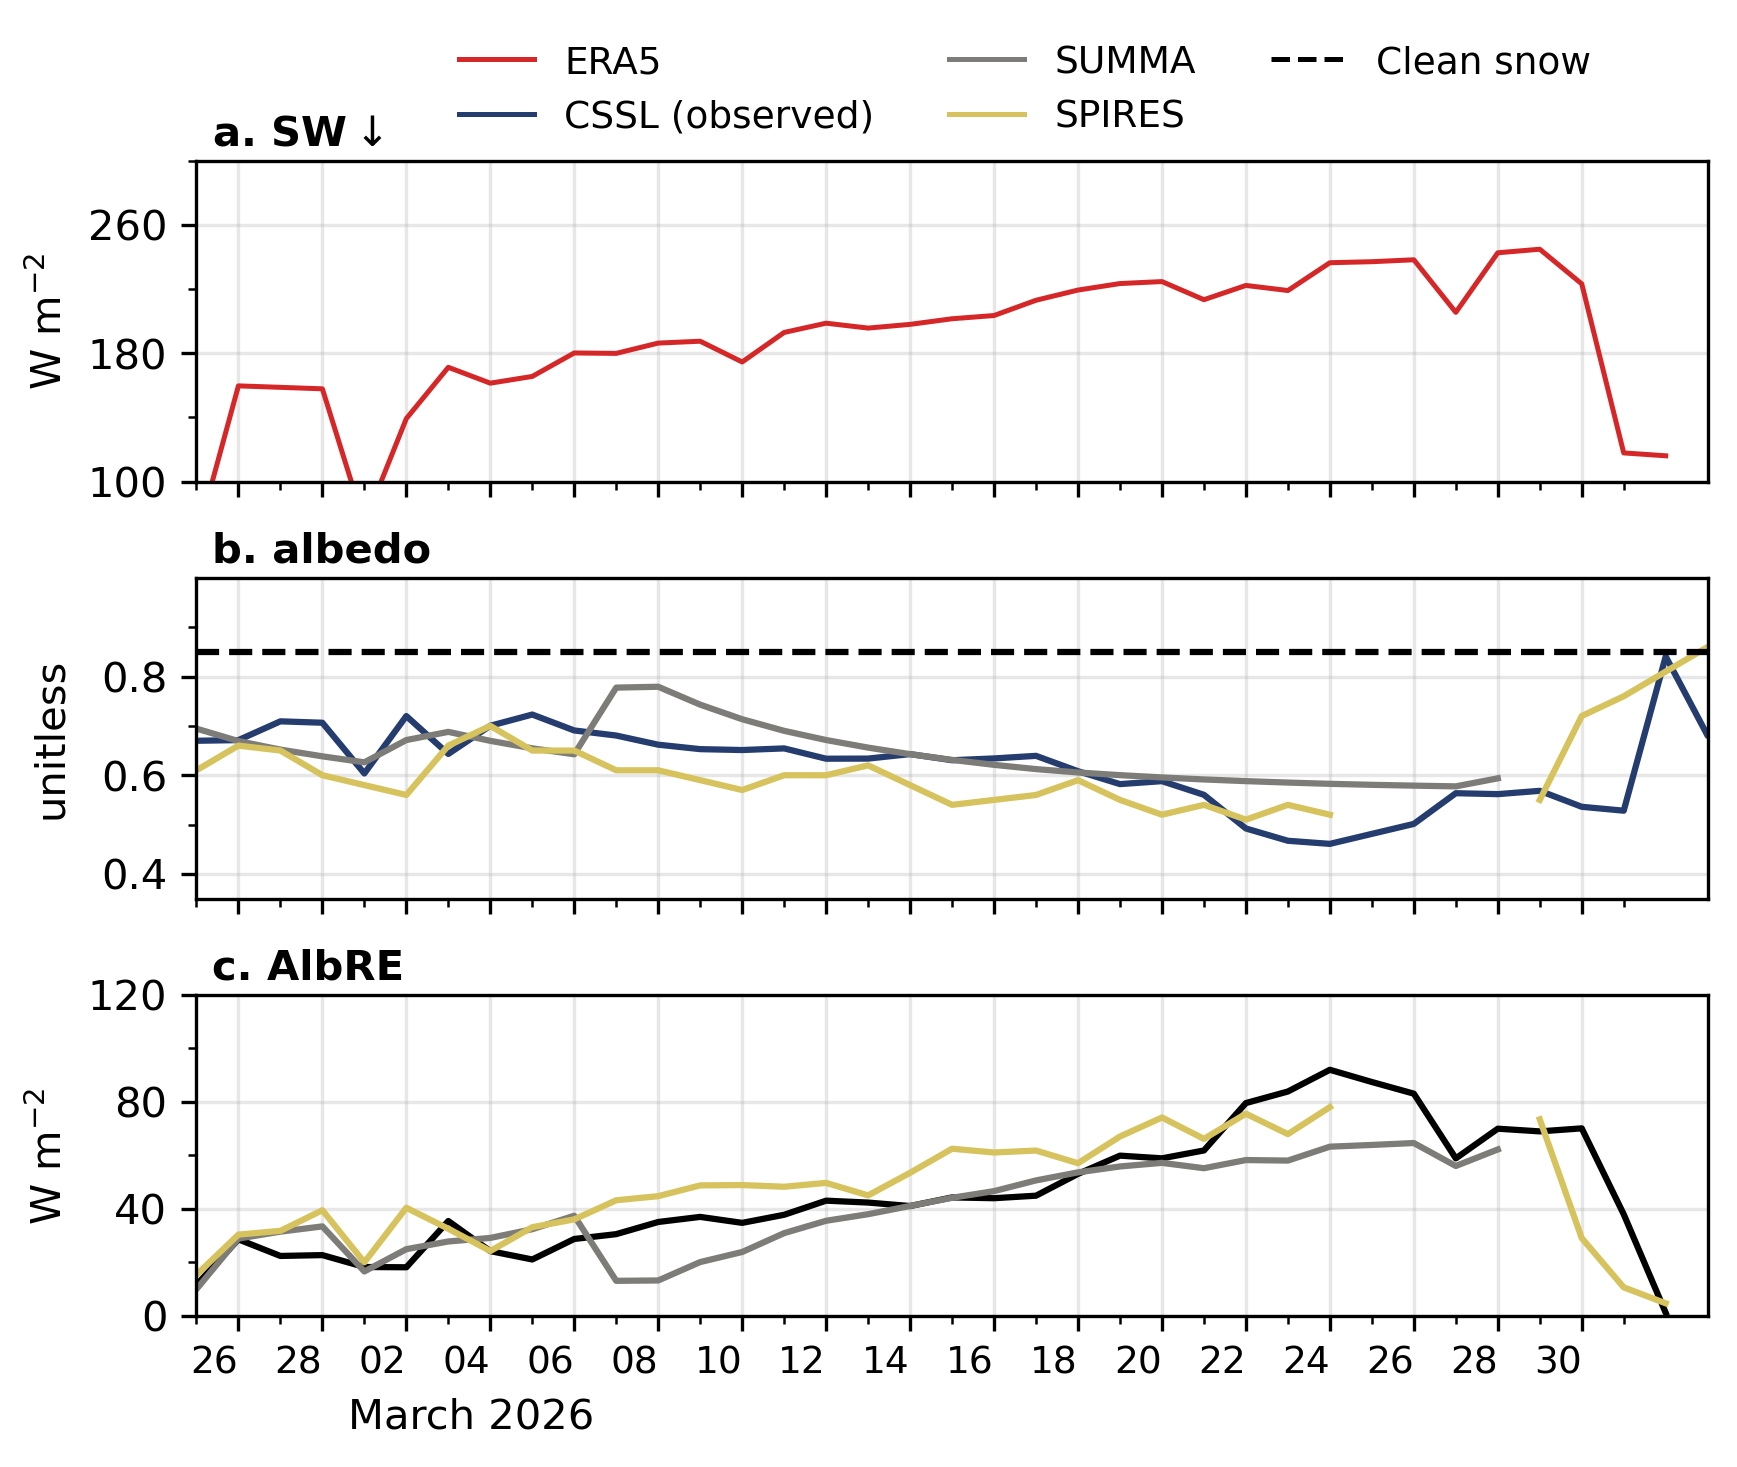
\includegraphics{images2/albedo_feedback_contribution.png}
%   \caption{Factors explaining \swnet during the March heatwave at the open CSSL site.
%     (a) Solar insolation (\swdn) during heatwave,
%     (b) snow $\alpha$ observed by CSSL, modelled by SUMMA, and retrieved from SPIReS at the CSSL site,
%     (c) effective optical snow grain size retrieved by SPiRes,
%     and (d) AlbRF, or the difference between fresh snow \rnet and observed \rnet for each $\alpha$ product or observation.}
%   \label{fig:albedo}
% \end{figure}

\begin{figure}[htbp]
  \centering
  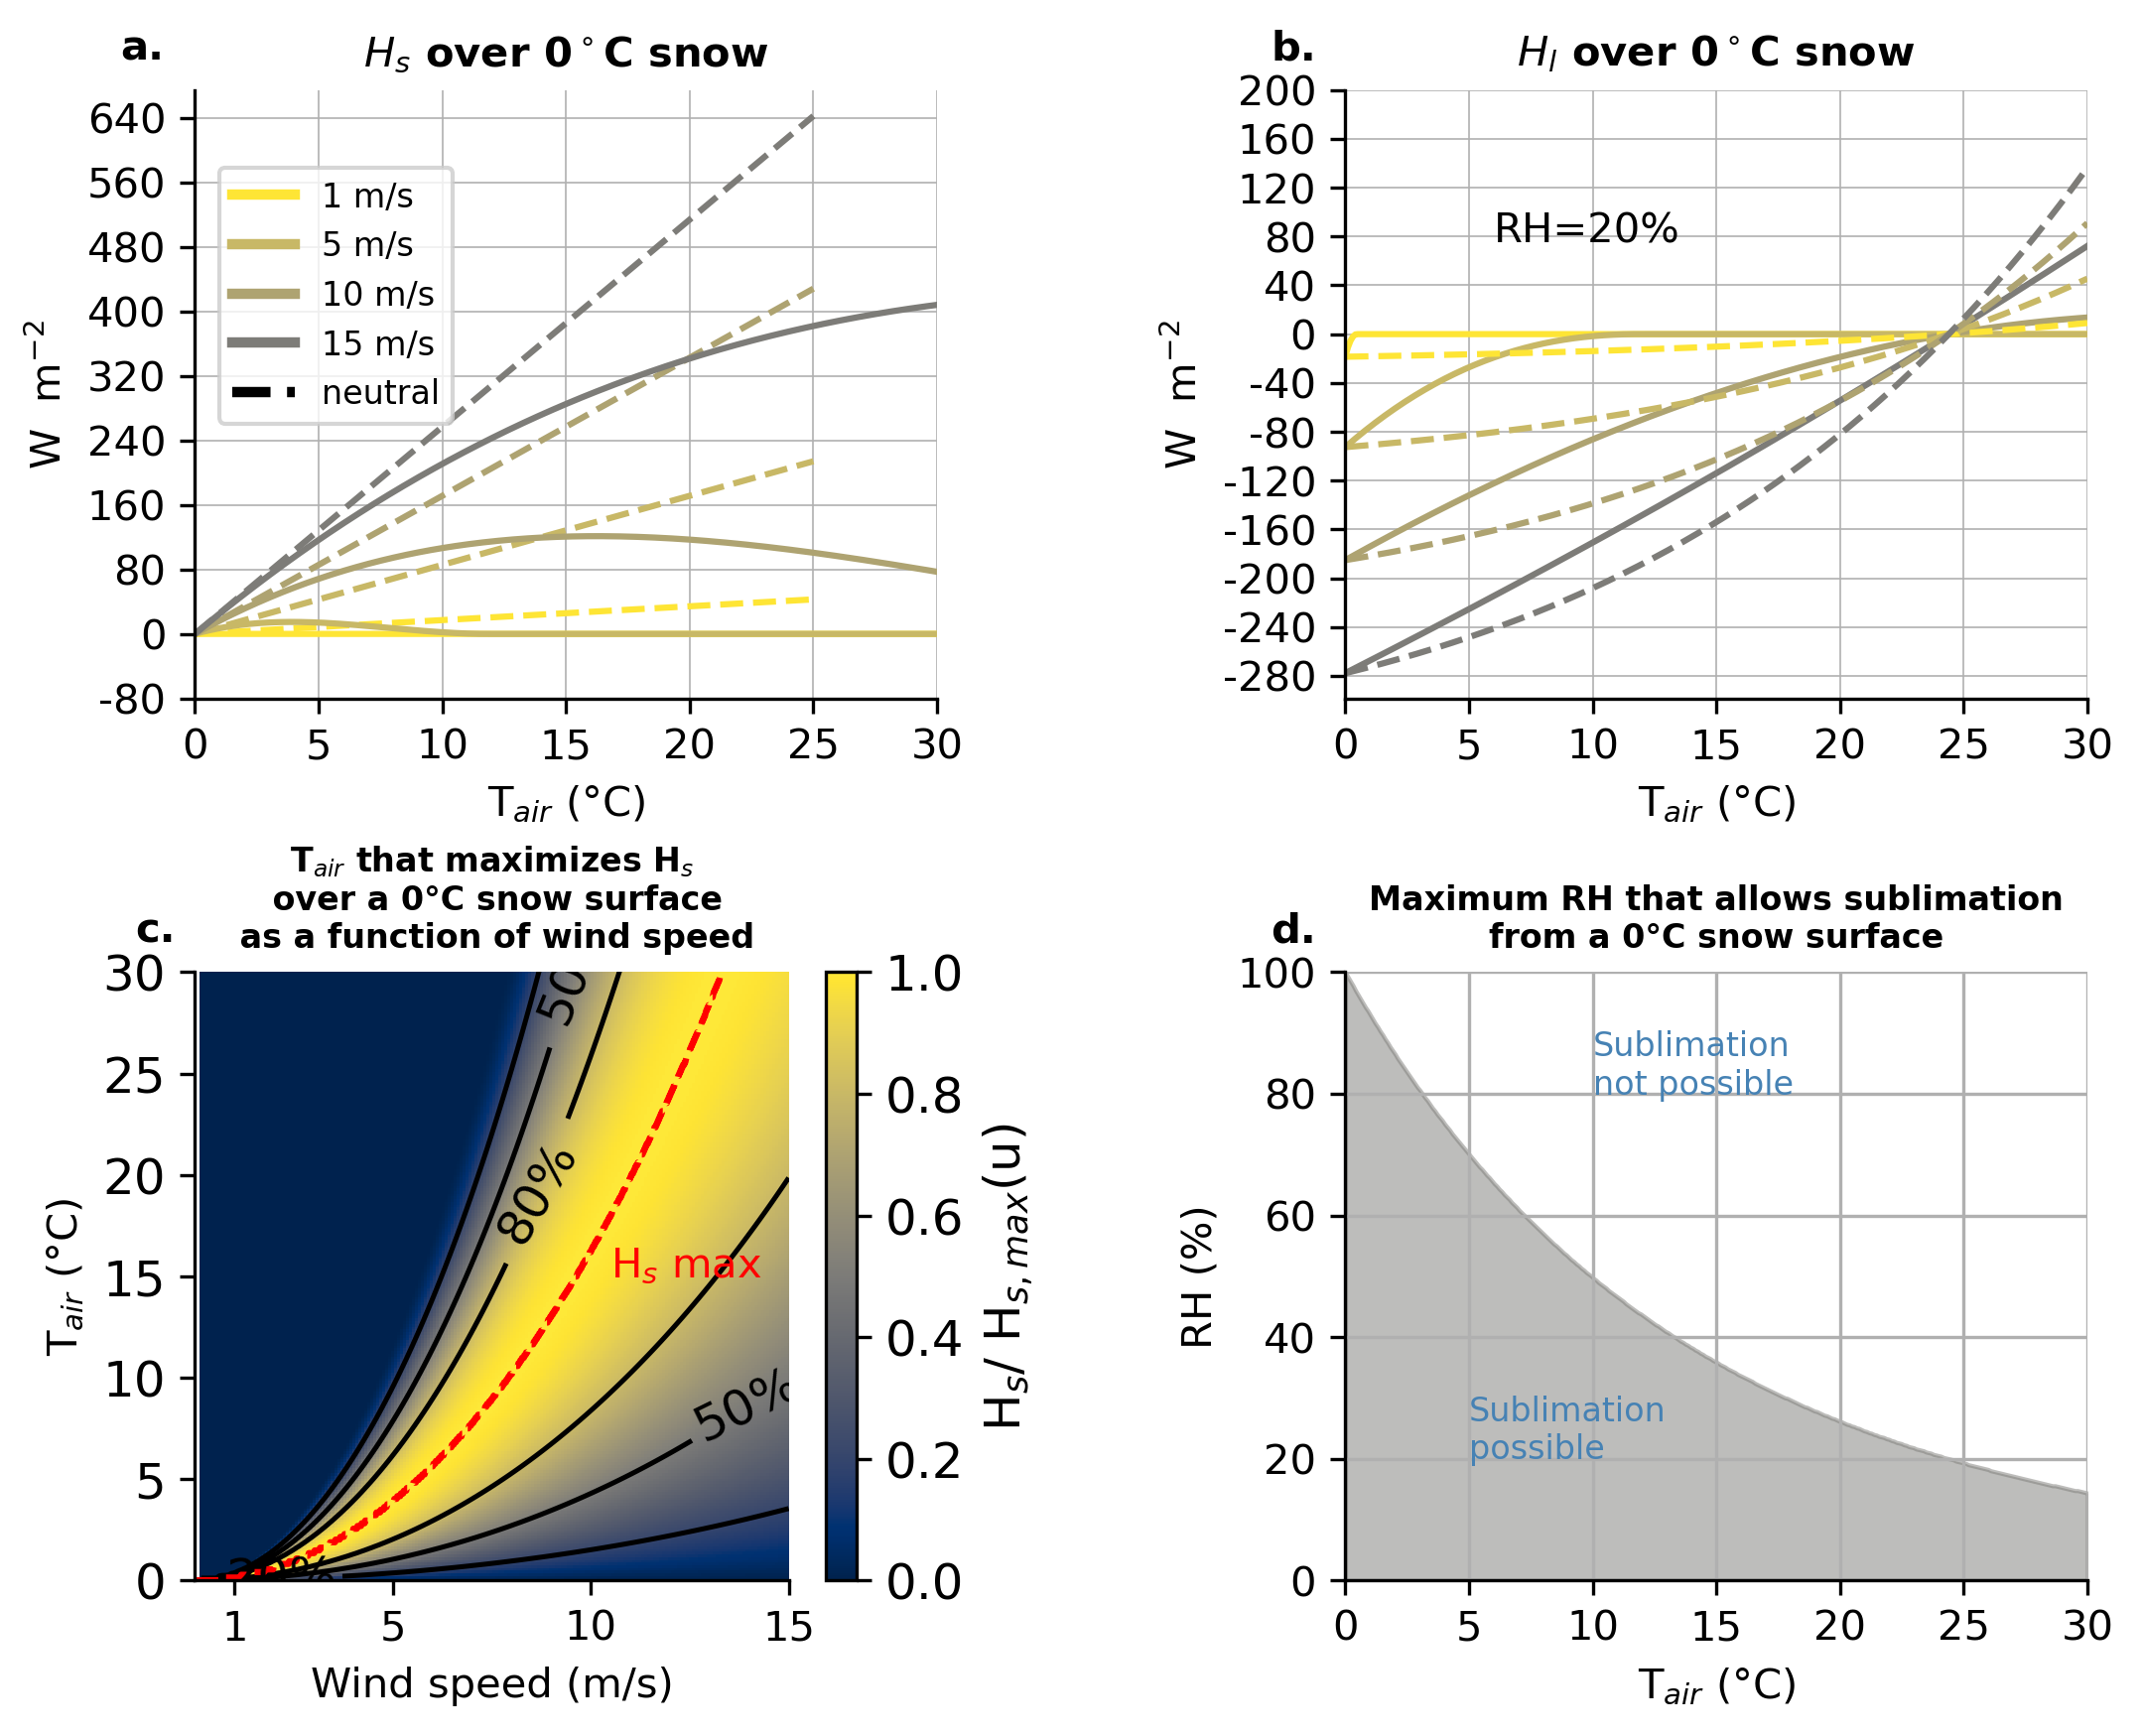
\includegraphics[width=.8\linewidth]{images2/idealized_sens_and_lat_heat.png}
  \caption{(a) Idealized sensible heat fluxes ($H_s$) into a melting snowpack as a function of \tair for four wind speeds (1, 5, 10, and 15 m s$^{-1}$) at a 12 m height for open-conditions and a snow surface roughness of z$_0$=0.002 m.
  Dashed lines show neutral-stability bulk transfer; solid lines show the same formulation with a stability correction applied as implemented in SUMMA.
  (b) the same as (a), but for $H_l$ with a fixed RH of 20\%.
  % (c) Clear-sky \lwnet as a function of \tair and RH over a 0\degrc snowpack using the \cite{Brutsaert1975-jl} formulation for \lwdn, and
  (c) The \tair that yields the maximum $H_s$ into a 0 \degrc snowpack after correcting for stability effects (dashed red line) for a given wind speed (u).
  Contours depict the fraction of the maximum $H_s$ for that wind speed value.
  (d) The thermodynamic limitation of sublimation as a function of \tair, depicting the maximum RH that permits sublimation from a 0 \degrc snowpack.
  }
  \label{fig:idealized_sens_heat}
\end{figure}



\begin{figure}[htbp]
  \centering
  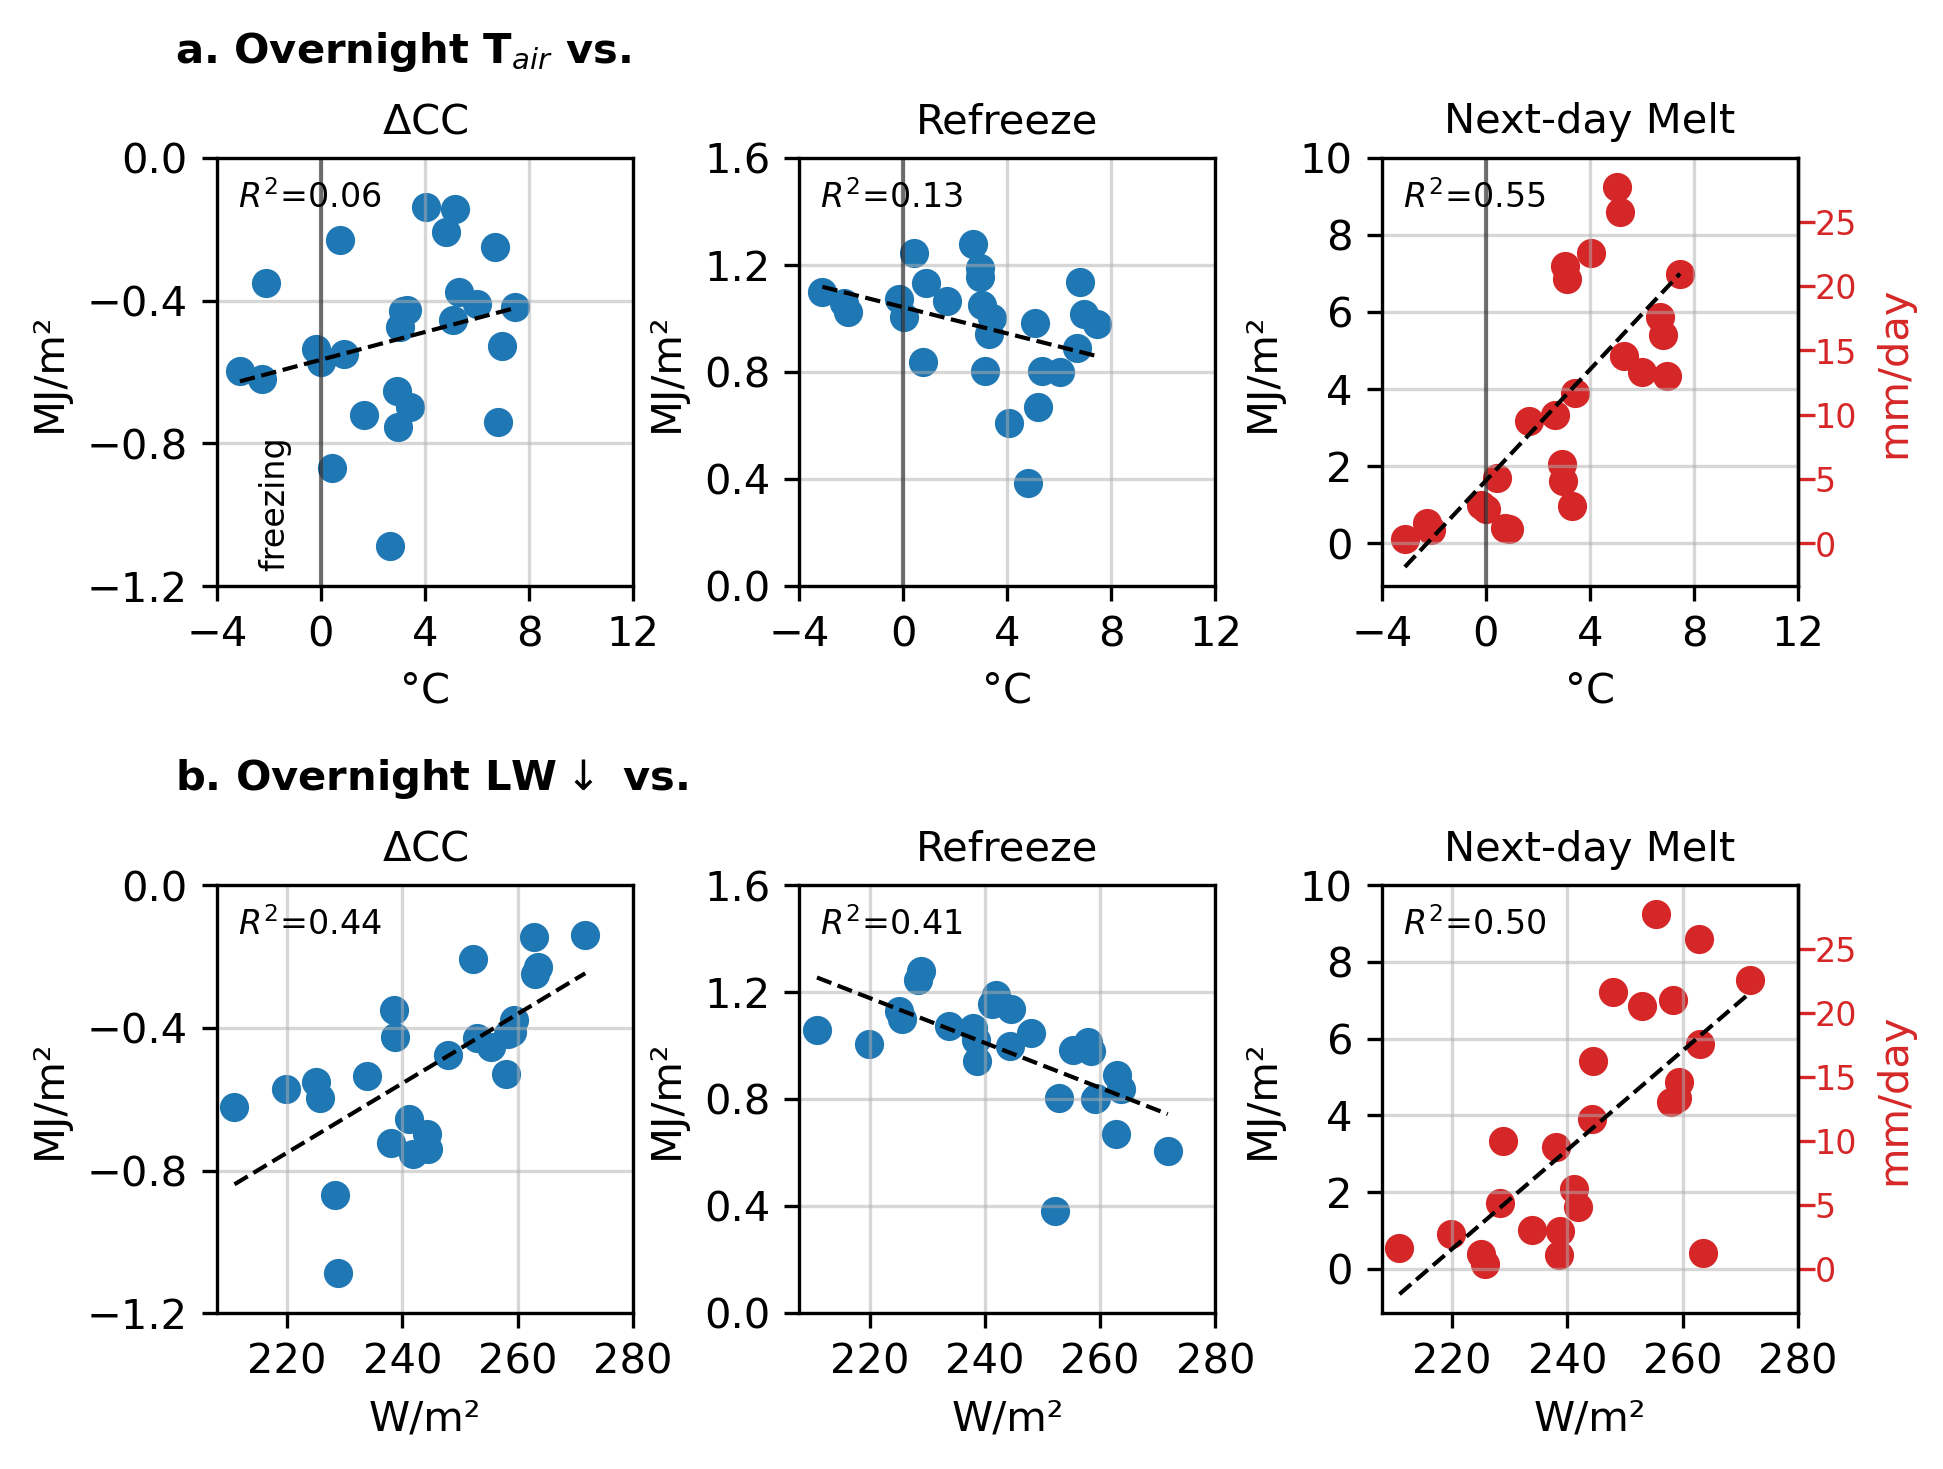
\includegraphics[width=\linewidth]{images2/overnight_freeze.png}
  \caption{The predictive power of overnight average \tair compared against overnight average \lwnet for \dcc, refreezing, and total melt during the next-day. 
  R$^2$ values and linear-regressions (dashed line) are depicted. 
  }
  \label{fig:overnight_tair}
\end{figure}




\clearpage


%%% WHOLE MONTH TABLE 
\begin{table}[h]
\centering
\caption{\todo{caption}: Forest and open-site energy balance terms (\mjmtwo; mm SWE equivalent in parentheses for H$_l$ and Melt) and cold content change (\mjmtwo) for March 2026 compared against the historical climatology (mean $\pm$ std).}
\label{tab:forest_open_summary}
\begin{tabular}{llrrrrrrr}
\toprule
 & & SW$_{net}$ & LW$_{net}$ & H$_s$ & H$_l$ & G & Melt & $\Delta$CC \\
\midrule
\multirow{3}{*}{Forest} & 2026 & 52.1 & 28.1 & 22.9 & -11.0 (-3.9) & 4.0 & 94.3 (282.4) & 0.0 \\
 & Mean & 37.0 & -2.2 & 7.7 & -22.5 (-7.9) & 2.7 & 34.4 (103.1) & 1.2 \\
 & Std & 16.4 & 19.4 & 19.2 & 15.8 (5.6) & 4.6 & 49.4 (147.8) & 2.8 \\
\midrule
\multirow{3}{*}{Open}   & 2026 & 229.3 & -127.5 & 39.7 & -0.7 (-0.2) & 4.3 & 142.1 (425.6) & 0.0 \\
 & Mean & 132.8 & -123.3 & 25.0 & -6.5 (-2.3) & 3.6 & 30.0 (89.9) & 2.0 \\
 & Std & 61.2 & 35.8 & 16.9 & 9.6 (3.4) & 6.3 & 64.1 (192.0) & 5.4 \\
\bottomrule
\end{tabular}
\end{table}


%%% DAY AND NIGHT TABLE 
\begin{table}[h]
\centering
\caption{Day/nighttime decomposition of Forcings (SW$_{net}$+LW$_{net}$+H$_s$+H$_l$+G), Melt/Refreeze, and $\Delta$CC, in \mjmtwo, for March 2026 compared against the historical climatology (mean $\pm$ std).}
\label{tab:forest_open_diel_summary}
\begin{tabular}{llrrrrrr}
\toprule
 & & \multicolumn{2}{c}{Forcings} & \multicolumn{2}{c}{Melt/Refreeze} & \multicolumn{2}{c}{$\Delta$CC} \\
\cmidrule(lr){3-4} \cmidrule(lr){5-6} \cmidrule(lr){7-8}
 & & Day & Night & Day & Night & Day & Night \\
\midrule
\multirow{3}{*}{Forest} & 2026 & 105.4 & -9.2 & 101.9 & -7.5 & 1.7 & -1.7 \\
 & Mean & 49.2 & -26.6 & 50.5 & -16.0 & 12.2 & -11.0 \\
 & Std & 47.0 & 19.8 & 49.5 & 14.0 & 17.6 & 16.9 \\
\midrule
\multirow{3}{*}{Open}   & 2026 & 189.2 & -44.1 & 172.1 & -29.9 & 11.9 & -11.9 \\
 & Mean & 71.5 & -39.9 & 49.2 & -19.1 & 23.5 & -21.5 \\
 & Std & 66.6 & 23.1 & 72.4 & 16.9 & 19.8 & 20.8 \\
\bottomrule
\end{tabular}
\end{table}


% \caption{Data displayed in Figure \ref{fig:monthly_seb_mar} presented as a table. 
% Equivalent units of mm of SWE for \hlat and Melt are presented in parentheses. 
% The March 2026 change in SWE ($\Delta$ SWE) and historical mean and standard deviation are also presented.
% }






\clearpage

% --- BIBLIOGRAPHY ---
% \bibliographystyle is set to apacite by agujournal2019.cls
\bibliography{paperpile} % Ensure paperpile.bib is in the same folder
\end{document}
